\documentclass[oneside,11pt]{memoir}

% Fonts
\usepackage[T1]{fontenc}	% better output encoding
\usepackage{lmodern}		% Latin Modern instad of CM
\usepackage{inconsolata}	% better monospaced font
\usepackage{microtype}		% fix the little things % comes after any fonts

% basics
\usepackage[textwidth=0.65\paperwidth]{geometry}	% Adjust margins
\usepackage{graphicx}	% now you can add pretty pictures
\usepackage{url} 		% makes urls look nicer
\usepackage[usenames,dvipsnames]{color} % adds colored text
\usepackage[font=footnotesize]{caption}	% more control over figure captions
\usepackage{xparse}		% nesting arguments wtihin environments
\usepackage{underscore}	% better text underscores, defua
\usepackage{marginnote}	% better margin notes
\usepackage{tabularx}	% more flexible tables
\usepackage[table]{xcolor}	% alternating table colors
\usepackage{todonotes}	% backend organization. Also for some reason necessary for tikz

% Complex packages
\usepackage{tcolorbox} 	% frames
\usepackage{listings} 	% allows for adding $ at the beginning of lines
\usepackage{dirtree}	% pretty directory trees

% Lists
\usepackage[ampersand]{easylist}	% Nicer syntax for creating lists
\usepackage{paralist}	% Allows inline lists
\usepackage[modulo,right]{lineno}	% right-hand line numbers


% Hyperref
\usepackage[colorlinks=true]{hyperref} 	% allows hyperlinking % NEEDS TO BE LOADED LAST

% underscore defaults to text mode over math mode
\catcode`_=12 

% Document information
\title{Using GNU \texttt{make} for Neuroimaging Workflow}
\author{ Tara M. Madhyastha (\url{madhyt@uw.edu}) \and Zo\'e Mestre (\url{zlm@uw.edu}) %
	\and Trevor K. McAllister-Day (\url{tkmday@uw.edu}) \and Natalie Koh (\url{natkoh@uw.edu)} %
}

% Set up the margins and the mymarginnote command
\setlrmargins{*}{*}{1}
\setmarginnotes{0.25in}{1in}{0.5in}
\checkandfixthelayout

\newcommand{\mymarginnote}[2]{\marginpar{{\small \sffamily \selectfont\fbox{\textbf{#1}} #2}}} % custom margin notes

% Code display commands
\newcommand\maken{\texttt{make}} % typeset 'make' always in monospace
\newcommand\bashn{\texttt{bash}} % same for 'bash'

\definecolor{textgray}{gray}{0.75}
\makeatletter
\newcommand{\onelbox}[2]{%
	\setbox0=\hbox{#1}%
	\setlength{\@tempdima}{\dimexpr\wd0+13pt}%
	\begin{tcolorbox}[colback=#2,boxrule=0.5pt,arc=4pt,
		left=6pt,right=6pt,top=6pt,bottom=6pt,boxsep=0pt,width=\textwidth]
		#1
	\end{tcolorbox}
}
\makeatother

% ONE-LINE environments
% $ is automatically added to the bash prompt.
% % \hfill\, forces the minipage onto a new line. Don't ask.
\newcommand{\bashcmd}[1]{ \hfill\, \begin{minipage}[t]{\linewidth}  \hrule \vspace{0.5\baselineskip} \texttt{\small \$ #1} \vspace{0.5\baselineskip} \hrule \end{minipage} \vspace{0.5\baselineskip} }
\newcommand{\makecmd}[1]{ \vspace{0.5\baselineskip} \onelbox{\texttt{\small #1}}{white} \vspace{0.5\baselineskip} }
% Since these commands are embedded in floats, the nicest way to space them properly in the output
% % is to make sure that there is a newline between the command and the text you want to follow the figure.

% load languages for the listings class
\lstloadlanguages{bash,make}

% DEFINE BASH MULTILINE ENVIRONMENT
\makeatletter
% define custom macro that expands to the language name
% (for comparison purposes)
\newcommand\langname@bash{}
\def\langname@bash{bash}
% define custom prompt
\newcommand\prompt@bash{\$\ }
% define a macro (initially empty) and insert it at the beginning of every paragraph
\newcommand\addedToEveryPar@bash{}
%\lst@AddToHook{EveryPar}{\addedToEveryPar@bash}
% redefine the macro by the custom prompt, but only if the language in use
% be `bash'
\lst@AddToHook{PreInit}{%
	\ifx\lst@language\langname@bash%
	\let\addedToEveryPar@bash\prompt@bash%
	\fi
}
\makeatother
\lstnewenvironment{bashsession}[1][]{\lstset{language=bash,gobble=8,basicstyle=\small\ttfamily#1}}{}

\newenvironment{bash}[2] % 
{ \begin{samepage} \begin{figure}[h!] \def\captiontext{#1} \def\labelt{#2} \vspace{0.5\baselineskip} \hrule \vspace{0.5\baselineskip} \ttfamily } { \vspace{0.5\baselineskip} \hrule \vspace{0.5\baselineskip}  \caption{\captiontext} \label{\labelt} \end{figure} \end{samepage} } 

% % This is rather unfortunate, but you can't nest \lstnewenvironment inside a \newenvironment so inorder to typset a block of bash code use :
% % 	\begin{bash}\begin{bashsession}
% %			multi-line
% %			code
% %		\end{bashsession}\end{bash}

% DEFINE MAKE MULTILINE ENVIRONMENT
\newenvironment{make}[2] %
{ \begin{figure}[h!] \def\captiontext{#1} \def\labelt{#2} \begin{tcolorbox}[colback=white,boxrule=0.5pt,arc=4pt,left=6pt,right=6pt,boxsep=0pt,width=\textwidth] \ttfamily } { \normalfont \end{tcolorbox} \caption{\captiontext} \label{\labelt} \end{figure} }
% You must terminate lines in the make environment
% To indent lines, use \tab

% use \maker to create recipes
\newcommand{\maker}[2]{\textcolor{blue}{#1}:\enspace#2}

% tab for indenting in make environment
\newcommand{\tab}{\hspace*{4em}}

% DEFINE MAKE REALLY LONG INPUT
\newenvironment{makefileread} %
{ \pagestyle{empty}\small\ttfamily\setlength{\parindent}{0pt} } %\newgeometry{scale=0.85, centering}
{ \pagestyle{ruled}\normalsize\normalfont\setlength{\parindent}{17pt} } %\restoregeometry\

% Specify command for "--"
% use this to specify bash long inputs (--) so they don't get swallowed up into hyphens.
% No space follows by default
\newcommand{\dd}{-{}-} 

% This is a better-looking #, I think
\newcommand{\mypound}{\protect\scalebox{0.8}{\protect\raisebox{0.4ex}{\#}}}

% % SOURCE CODE HIGHLIGHTING
\newcounter{codehighlight}
\newcommand*{\lnum}[1]{\tikz[baseline=(char.base)]{	\node[shape=circle,draw,inner sep=0.8pt, fill=black, text=white] (char) {\rmfamily\bfseries\footnotesize#1}; } }
\newcommand*{\lnote}{\stepcounter{codehighlight}\llap{{\lnum{\thecodehighlight}}\hskip 6em}}

% Change numbering
\setsecnumdepth{chapter}	% only number chapters
\maxtocdepth{subsection}	% put subsections in the table of contents
\makeatletter
\@addtoreset{chapter}{part}	% reset the chapter counter at each part
\makeatother

\pagestyle{ruled}	% Graphics command
\raggedbottom		% Allow more flexibility at the bottom of the page - helpful with lots of floats.

%\def\hrulefill{\leavevmode\leaders\hrule height 2pt\hfill\kern\z@}
\newcommand{\lmhrule}{{\color{gray!75} \rule{\textwidth}{2pt}}\\}

\begin{document}
	
	% Cover page
	
	\thispagestyle{empty}
	\begin{vplace}[0.7]
		\begin{center}
			
\includegraphics[width=0.75\linewidth, natwidth=1890, natheight=761]{IBIClogo.png}				% IBIC logo
			\vspace{0.25in} \hrule \vspace{0.25in}															% vspace + hrule
			{ \fontsize{30pt}{36pt} \selectfont Using GNU \textsc{make} for Neuroimaging Workflow\par }		% Title
			\vspace{0.25in} \hrule \vspace{0.25in}															% vspace + hrule
			{\LARGE University of Washington} 																% University of Washington	
		\end{center}	
	\end{vplace}
	
	\frontmatter	% Define the front matter section of the document
	
	\maketitle		% Title page
	
	\tableofcontents
	
	\listoffigures
	
	\mainmatter		% The actual content
	
	\part{Manual}
	
	\chapter[Introduction to \maken{}]{A Conceptual Introduction to \maken{} for Neuroimaging Workflow}
\label{chap:intro}
	
This guide is intended for scientists working with neuroimaging data (especially a lot of it) who would like to spend less time on workflow and more time on science. The principles of automation and parallelization, taken from computer science, can easily be applied to neuroimaging to make certain parts of the analysis go quickly so that the computer can do what it's best at. This kind of automation supports reproducible science (or at the very least, allows you to rerun your analysis extremely quickly with a variant of the processing stream, or on a new dataset).
	
Over the last few years we have developed neuroimaging workflows using \maken, a program from the 1970s that was originally used to describe how to compile and link complicated software packages. It is an amazing program that is still in use today. It is fairly easily repurposed to describe neuroimaging workflows, where you specify how you ``make'' one file, which can depend on several other files, using some set of commands. Once you have expressed these ``rules'' or ``recipes'' in a file (a Makefile), you actually have a fully parallelizable program, which allows you to run the Makefile over as many cores as you have (or on a Sun Grid Engine). This has been done before: FreeSurfer incorporates \maken{} into their pipeline ``behind the scenes.''  We have developed many examples of neuroimaging pipelines in multiple domains that are written using \maken{}.
	
Modern tools for neuroimaging workflow (nipype, LONIPipeline) incorporate data provenance (e.g., information about how and when the results were generated), wrappers for arguments so that you do not need to worry about all the different calling conventions of programs, and generation of flow graphs. However, \maken{} allows expression of neuroimaging workflow with only the programming concepts of parallelism and variables. Being able to incorporate programs from many different packages without wrapping them saves time and effort.  T.\,M. has taught several undergraduates, graduates and staff to use it to develop, debug, and execute pipelines. It is simple enough that the basic concepts can be understood by non-programmers. This results in more time teaching and doing neuroimaging than teaching (and doing) programming.
	
\section{Conventions Used in This Manual}
	
By convention, actual commands or filenames will be typeset in Inconsolata (for example, \texttt{ls}, \texttt{make}, FSL's \texttt{bet}, and \texttt{flirt}.) Makefile examples will also be typeset in Inconsolata.
	
Commands to be executed in a shell (we assume \bashn{} throughout this manual) are written on a line beginning with a dollar sign (\$) \mymarginnote{!}{You do not type the \$ to execute \bashn{} commands; it stands for the prompt.}and displayed between two horizontal lines, as follows:	
\bashcmd{echo Hello World!}	
	
Examples of commands from Makefiles are shown in an outlined box with no special prompt character:
\makecmd{This is a make command.}
Additionally, recipes are easily identified by their opening syntax, where the recipe target is usually rendered in blue (see \autoref{make:syntax} or \autoref{make:recipe1}).	
	
Data for the lab practicals and examples documented in this manual are available from NITRC. We will assume that you have downloaded them into some location on your own machines (e.g. \texttt{~makepipelines}) and will refer to these files directly. To run the example makefiles, you must set an environment variable, \texttt{MAKEPIPELINES} to the location of this directory (see \autoref{chap:examples}). If you are at IBIC you may find these examples on \texttt{/project_space/makepipelines}.%%% MUST PUT NAME HERE

Throughout this manual we assume a UNIX style environment (e.g., Linux or MacOS) with common neuroimaging packages installed. All examples have been tested on Debian Wheezy using GNU Make 3.81. Please let us know of problems or typos, as this manual is a work in progress.
	
\section{Quick Start Example}
\mymarginnote{!}{Recipes in \maken{} need to begin with a TAB character. Not eight spaces, not nine, but exactly one TAB character.}
	
A makefile is a text file created in your favorite text editor (e.g., \texttt{txtedit}, \texttt{emacs}, \texttt{vi}, \texttt{gedit} -- \emph{not} Office or OpenOffice). By convention, it is typically called ``Makefile'' or ``foo.mk'' (i.e., it has a .mk extension). It is like a little program that is run by the program \maken{}, in the same way that a shell script is program run by the program \texttt{/bin/bash}.
	
A makefile contains commands that describe how to create files from other files (for example, a skull-stripped image is created from the raw T1 image, or a T1 to standard space registration matrix is created from a standard space skull-stripped brain and a T1 skull-stripped brain).
	
These commands take the form of ``rules'' that look like those in \autoref{make:syntax}.
	
\begin{make}{Basic \maken{} syntax. }{make:syntax}
	\maker{target}{dependencies} \\
	\tab \begin{minipage}[t]{\linewidth-4em} {\color{gray} Shell commands to create target from dependencies (a recipe), beginning with a [TAB] character.} \end{minipage}
\end{make}
	
This may be best understood by example. \autoref{make:recipe1} is a simple makefile that executes FSL's \texttt{bet} command to skull-strip a T1 nifti.
	
\begin{make}{A very basic \maken{} recipe.}{make:recipe1}
	\maker{s001\_T1\_skstrip.nii.gz}{s001\_T1.nii.gz} \\
	\tab bet s001_T1.nii.gz s001_T1_skstrip.nii.gz -R
\end{make}
	
In \autoref{make:recipe1} the target file is \texttt{s001_skstrip.nii.gz}, which ``depends'' on \texttt{s001_T1.nii.gz}. More specifically, to ``depend on'' something means that \begin{inparaenum}[\itshape a)\upshape] \item it cannot be created unless the dependency exits, and \item it must be recreated if the dependency exists, but is newer than the target. \end{inparaenum}
	
The ``recipe'' is the \texttt{bet} command that creates the skull-stripped image from the T1 image. This executes in a shell, just as if you were typing it in the terminal.
	
If this rule is saved inside a file called \texttt{Makefile} in the same directory as \texttt{s001_T1.nii.gz}, then you can create the target as follows:	
\bashcmd{make s001_T1_skstrip.nii.gz}
	
Alternatively, in this instance, you could call:
\bashcmd{make}	
	
If you specify a target as an argument to make, it will create that target. If you do not, \maken{} will build the first target in the file. In this case, they are the same.
	
\section{A More Realistic Example}
	
In the example above, we specified exactly what file to create and what file it depended upon. However, in neuroimaging analyses we normally have many subjects and want to do the same things for all of them. It would be a royal pain to type in every rule to create every file explicitly, although it would work. Instead we can use the concepts of variables and patterns to help us. 
A variable is a name that is used to store other things. You can set a variable to something and then refer to it later. A pattern is a substring of text that can appear in different names.
Suppose we have a directory that contains the T1 images from 100 subjects with identifiers s001 through s100. The T1 images are named \texttt{s001_T1.nii.gz}, \texttt{s002_T1.nii.gz} and so on. This makefile will allow you to skull strip all of them (and on as many processors as you can get a hold of (see \autoref{chap:parallel}) but I'm getting ahead of myself here).
	
\begin{figure}[h!]
	\begin{center}
		\begin{tabular}{ r l }
			\texttt{\%} 	& matches a pattern. \\
			\texttt{\$@}	& is the target. \\
			\texttt{\$<}	& is the first dependency. \\
			\texttt{\$(VAR)}& is a \maken{} variable.
		\end{tabular}
	\end{center}	
	\caption{Automatic \maken{} variables}
\end{figure}

The first two lines in \autoref{make:recipe2} set variables for Make. Yes, the syntax is icky but it is well explained in the GNU \maken{} manual. We will summarize here. The first variable is assigned to the result of a ``wildcard'' operation that expands to all files with the pattern \texttt{s????_T1.nii.gz}. If you are not familiar with wildcards, if you do a directory listing of that same pattern, it will match all files that begin with an ``s,'' are followed by exactly three characters, and then ``_T1.nii.gz.'' In other words, the \texttt{T1files} variable is set to be all T1 files belonging to those subjects in the current directory.
	
\begin{make}{A more realistic example}{make:recipe2}
	T1files=\$(wildcard s???_T1.nii.gz) \\
	T1skullstrip=\$(T1files:\%_T1.nii.gz=\%_T1_skstrip.nii.gz) \\
	\maker{all}{\$(T1skullstrip)} \\
		
	\maker{\%_T1_skstrip.nii.gz}{\%_T1.nii.gz}\\
	\tab bet \$< \$@ -R
\end{make}
	
The second variable is set using pattern substitution on the list of T1 files, substituting the file ending (\texttt{_T1.nii.gz}) for a new file ending (\texttt{_T1_skstrip.nii.gz}) to create the list of target files. Note that the percent sign (\texttt{\%}) matches the subject identifier. It is necessary to use the percent sign to match only the subject identifier (and not the subject identifier plus the following underscore, or some other extension) when matching parts of file names in this way. 
	
We have now introduced a new type of rule (\texttt{make all}) which has no recipe. Make will look for a file called \texttt{all} and this file will not exist. It will then try to create all the things that all depends on (and those files, the skull stripped images, don't exist either). So it will then take names of each skull stripped file, one by one, and look for a rule to make it. When it has done that, it will execute the (nonexistent) recipe to make target \texttt{all} and be finished. Because the file \texttt{all} still does not exist (by intention), trying to make the target will always result in trying to make all the skull stripped files.
	
This brings us to the final rule. The percent sign in the target matches the same text in the dependency. This target matches the name of each of the skull stripped files desired by target all. So one by one, they will be created. In the recipe for the final rule, we have used a shorthand of \maken{} to refer to both the dependency that triggered the rule (\texttt{\$<}) and the target (\texttt{\$@}). We do this because since the rule is generic, we do not know exactly what target we are making. However, we could also write out the variables (as seen in \autoref{make:recipe3}).
	
\begin{make}{An expansion of \autoref{make:recipe2}}{make:recipe3}
	\maker{\%_T1_skstrip.nii.gz}{\%_T1.nii.gz} \\
	\tab bet \$*_T1.nii.gz \$*_T1_skstrip.nii.gz -R
\end{make}
	
In this version of the rule, we use the notation \texttt{\$*} to refer to what was matched in the target/dependency by \texttt{\%}. If the previous version looked to you like a sneeze, this may be more readable.
	
Now you can run this makefile in many ways. As before, to create a specific file, you can type:	
\bashcmd{make s001_T1_skstrip.nii.gz}
	
To do everything, you can type: \texttt{make all} or just \maken{}.
	
Suppose you do this and later find that the T1 for subject 036 was not properly cropped and reoriented. You regenerate this T1 image from the dicoms and put it in this directory. Now if you type make again, it will regenerate the file \texttt{s036_T1_skstrip.nii.gz}, because the skull strip is now older than the original T1 image. Suppose you acquire four more subjects. If you dump their T1 images into this directory following the same naming convention and type \maken{}, off you go.

This probably seems like an enormous amount of effort to go to for some skull stripping. However, the benefit becomes clearer as the complexity of the pipelines increases.
	
\section{What is the Difference between a Makefile and a Shell Script?}
	
This is a really good question. A makefile is basically a specialized program that is good at expressing how X depends upon Y and how to create it. The recipes in a makefile are indeed little shell scripts, adding to the confusion. By making these dependencies explicit, you enable the computer to execute as many of the recipes as it can at once, finishing the work as quickly as possible. It allows the computer to pick right back up if there is a crash or error that  causes the job to die somewhere in the middle. It allows you, the scientist, to decide that you want to change some step three-quarters of the way down and redo everything that depends upon that step.
	
Shell scripts are more general programs that can do all sorts of things, but inherently do them one at a time. For example, the shell script that is the equivalent to \autoref{make:recipe2} could be written something like \autoref{bash:makefile}.
	
\begin{bash}{A makefile expressed in \bashn{}}{bash:makefile}
	\#!/bin/bash \\
	for i in s???_T1.nii.gz \\
	do \\
	name=\`{}basename \$i .nii.gz\`{} \\
	bet \$i \${name}_skstrip.nii.gz -R \\
	done
\end{bash}
	
There is nothing in this script to explicitly tell the computer that each individual T1 image can be processed independently of the others; the order does not matter. So if you are on a multicore computer that can execute many processes at once, you could not exploit this parallelism with this shell script. Furthermore, you can see that to add a few subjects or redo a few subjects, you will need to edit the script to avoid rerunning everyone. 
	
If you have ever found yourself writing a shell script to do a large batch job, and then commenting out some of the subject identifiers to redo the few that need redoing, then commenting out some other parts and adding new lines to the program, and so forth, you are dealing with the problems that \maken{} can help with. If you are not convinced, see \autoref{sec:practicum1} for a more detailed explanation of how \maken{} works. 	% Introduction to make
	
	\chapter{Running \maken{} in Context}
\label{chap:context}

In the previous chapter we presented some toy examples. However, in real neuroimaging life one deals with hundreds of subjects with multiple types of scans and many planned analyses. To keep this straight requires some conventions, whether you use \maken{} or not. Here we describe some conventions that are useful for managing realistic projects.

\section{File Naming Conventions}
\label{sec:naming}

File naming conventions are critical for scripting in general, and for Makefiles in particular. \maken{} is specifically designed to turn files with one extension (the extension is the last several characters of the filename) into files with another extension. For example, in \autoref{make:recipe1} we turned a file with an extension ``T1.nii.gz'' into a file with the extension ``T1_skstrip.nii.gz.'' 
\mymarginnote{!}{``\textbf{Extension}'' often refers to the file suffix, e.g., ``.csv,'' but there is no reason it must be limited to a fixed number of characters after a period.}

So we can use naming conventions within a project, and across projects consistently to reuse rules that we write for common operations. In fact, \maken{} has many built-in rules for compiling programs that are absolutely useless to us. But we can write our own rules.

Thus, it is important to decide upon naming conventions. 

\subsection{Subject Identifiers}

The first element of naming conventions is the subject identifier. This is usually the first part of any file name that we might end up using outside of its directory. For example, we might include the subject identifier in the final preprocessed resting state data, allowing us to dump all those files into a new directory for subsequent analysis with another program, without having to rename them or risk overwriting other subject files. Some features (by no means exhaustive) that may be useful for subject identifiers are:

\begin{easylist}[enumerate]
	& \textbf{They should contain some indicator of which project the subjects belong to.} \\
	This is particularly important if you work on multiple projects, or if you may be pooling data from multiple studies. Typically choose a multi-letter code that is the prefix to the subject ID.
	& \textbf{If applicable, they should contain some indicator of treatment group that the subject belongs to.} \\
	It is helpful to indicate in the subject ID (usually with another letter or digit code) whether the subject is part of a treatment group or a control.
	& \textbf{They should be short.} \\
	Short names are easier to type and to remember, and make it easier to work with lists of directories that are named according to the subject id.
	& \textbf{They should be the same length.} \\
	This is not necessary but helpful for pattern matching using wildcards in a variety of contexts within \maken{} and without.
	& \textbf{They should sort reasonably in UNIX.} \\
	Many utilities ultimately require a list of filenames, which is easy to generate using wildcards and the treatment group code if the subject ID sort order is reasonable. The classic problem is to name subjects S1 \ldots S10, S11 -- the subjects will not be in numeric order without zero-padding to the subject numbers.
	& \textbf{They should be easy to type.} \\
	\bashn{} has many tricks to help you avoid typing, but when you have to type, the farther you have to move the longer it takes. Do you really need capital letters? 
	& \textbf{They should be easy to remember for short periods of time.} \\
	My attention span is very short when doing repetitive tasks; subject IDs that are nine-digit random numbers are harder to remember than subject IDs that are four letter random sequences. 
	& \textbf{They should be easy to divide into groups using patterns.} \\
	My favorite set of subject IDs were randomly generated four letter sequences that sounded like fake English words, making it easy to divide the subjects into groups of just about any size using the first letters and wildcards. This makes it very easy to test something on a subset of subjects. 
	& \textbf{They should be consistently used in all data sets within the project.} \\
	If the subject identifier is ``RC4101'' in a directory, it should not be ``RC4-101'' in the corresponding REDCap database\footnote{REDCap is the Research Electronic Data Capture web application that we use for storing subject-specific information} and ``101'' in the neuropsychological data. It is easier if everyone can decide upon one form of name.
\end{easylist}

\subsection{Filenames}

File naming conventions begin with converted raw data (nifti files derived from the original DICOMs, for example), and continue on for each level of processing. We find it helpful to give these files specific names and then to perform subject-specific processing within the subject/session directory. The filenames for a recent active project are shown in \autoref{table:filenames}, where the subject ID is ``RPI001.''

\rowcolors*{2}{gray!50}{white} 	% alternating row coloing, starting on row 2 (ignore header)
\def\arraystretch{1.2}	% with all the caps, this table gets a little crammed. 
\begin{figure}[h!]
	\begin{tabularx}{\linewidth}{ >\ttfamily l X } % >\ttfamily applies monospaced font to column 1
											% column 1 expands, and forces 2 to shrink and wrap
		\rowcolor{gray!75}
		\normalfont\textbf{Filename} 		& \textbf{Description} 	\\ \hline
		RPI001_T1_brain.nii.gz				& Skull stripped T1 MPRAGE image 	\\  
		RPI001_T1.nii.gz					& T1 MPRAGE image 					\\  
		RPI001_read.nii.gz					& Reading task scan 				\\  
		RPI001_read_rest.nii.gz				& Resting state scan for reading session	\\ 
		RPI001_read_fMRIb0_phase.nii.gz		& $B_0$ Field map phase image for reading session\\
		RPI001_read_fMRIb0_mag.nii.gz		& $B_0$ Field map magnitude image for reading session\\  
		RPI001_read_fMRIb0_mag_brain.nii.gz & Skull stripped $B_0$  magnitude image \\  
		RPI001_write.nii.gz					& Writing task scan 				\\  
		RPI001_write_rest.nii.gz			& Resting state scan for writing session	\\  
		RPI001_write_fMRIb0_phase.nii.gz	& $B_0$ Field map phase image for writing session\\
		RPI001_write_fMRIb0_mag.nii.gz		& $B_0$ Field map magnitude image for writing session\\  
		RPI001_write_fMRIb0_mag_brain.nii.gz	& Skull stripped $B_0$ magnitude image	\\ 
		RPI001_DTI.nii.gz					& DTI image 						\\ 
		bvecs.txt							& b-vectors for  DTI processing 	\\
		bvals.txt 							& b-values for DTI processing\\ \hline
	\end{tabularx}
	\caption{Example of good file naming conventions}
	\label{table:filenames}
\end{figure}

The specific file names chosen are not as important as consistency in the use of extensions and names, and documentation of what these files are and how they were processed. The more you can keep things the same between projects, the more Makefiles you will be able to reuse from one study to another with minimal changes. 

\section{Directory Structure}
\label{sec:dir}

Typically, we create a directory for each project. Within that project directory is storage for scripts, masks, data files from other sources (e.g., cognitive or neuropsychological data) and subject neuroimaging data. Subjects may have different timepoints or occasions of imaging data, as well as physiological data and task-related behavioral data.
An example hierarchy (for project Udall) is shown in \autoref{figure:udalldir}.

\begin{center}
	\begin{figure}[h!]
		\dirtree{%
			.1 /project_space/Udall.
			.2 bin\DTcomment{Holds \bashn{} scripts written for this project}.
			.3 R\DTcomment{Holds R scripts}.
			.3 tcl\DTcomment{Holds tcl scripts}.
			.2 data\DTcomment{Other sources of data for all subjects}.
			.2 lib\DTcomment{Holds things that are used by many scripts and analyses}.
			.3 makefiles\DTcomment{Makefiles for this project}.
			.3 networkROIs\DTcomment{A set of ROI masks for fMRI analysis}.
			.3 tractographyMasks\DTcomment{A set of masks for tractography analysis}.
			.2 freesurfer\DTcomment{Freesurfer (cortical thickness) runs}.
			.2 tbss\DTcomment{Group-level Tract-Based Spatial Statistics analyses}.
			.2 subjects\DTcomment{All subject data collected in neuroimaging sessions}.
			.3 SUBJECT\DTcomment{A specific subject}.
			.4 session1\DTcomment{Difference subject sessions}.
			.4 session2.
			.4 session3.
			.5 behavioral\DTcomment{Subject behavioral (e.g., task) data}.
			.5 Dicoms\DTcomment{Original dicoms}.
			.5 Parrecs\DTcomment{PAR/REC files, the native Philips scanner format}.
			.5 physio\DTcomment{Physiological data}.
			.5 xfm_dir\DTcomment{Registration files}.
			.3 session3/SUBJECT\DTcomment{Symbolic link to the subject/session3 directories}.
			.3 incoming\DTcomment{Zip files with subject data from the scanner.}.
		}
		\caption{An example of a project directory.}
		\label{figure:udalldir}
	\end{figure}
\end{center}

This directory is typically protected so that only members of the project who are permitted by the Institutional Review Board to access the data may \texttt{cd} into the directory, using a specific group related to the project. The setgid bit \mymarginnote{?}{The \texttt{setgid} bit on a directory ensures that files created here assume the group to which the directory belongs, and not the group to which the person creating them belongs.} is set on the project directory and the file permissions are set by default to permit group read, write, and execute permission for each individual so that files people create within the directory substructure are accessible by others in the project. 



The structure is set up for a longitudinal project, where each subject is imaged at separate time points (sessions). All subject data is stored under the directory subjects (under subdirectories corresponding to each session). However, because often it is convenient to conduct analyses on a single time point, we create a convenience directory at the top level (e.g., session3) which has symbolic links to all of the subjects' session 3 data. This can make it easier to perform subject-specific processing.

Notice that in the project directory, we also keep scripts that we write to process the data, other data files, and miscellaneous support files for workflow (in the \texttt{lib/} subdirectory). Your naming conventions may differ and there may be more categories than we have, but it is important to decide upon some structure that everyone agrees upon for the project. This makes it much easier to find things.

We find it useful to locate the results of some subject-specific processing (e.g. co-registration of files, subject-level DTI processing, subject-level task fMRI processing) in the subject/session directories. However, other types of analyses are more conveniently performed in directories (e.g. \texttt{freesurfer/}, \texttt{tbss/}) that are stored at the top level of the project.

Data files that are collected from non-neuroimaging sources are usually kept in text (tab or comma-separated) form in the \texttt{data/} directory so that scripts can find and use them (e.g., to use the subject age or some cognitive variable as a regressor in an analysis). We have found it very useful to document, manage, and merge this data very carefully, including the important QA variables that describe whether or not a subject's scan should be included in analyses.

Finally, note that we have a directory labeled \texttt{incoming}. This is a scratch directory (it could be a symbolic link to a scratch drive) for placing zip files that come from the scanner, that contain the dicoms for the scan, the Philips-specific PAR/REC files, the physiological data logged (used to correct functional MRI data for heart rate and respiration-related signal) and data from scanner tasks (e.g., EPRIME files).

\section{Setting up an Analysis Directory}
\label{sec:analysisdir}

Up until this point we have only seen little examples of makefiles that process subjects within a single directory. However, real studies include many subjects and many analyses; each analysis often produces hundreds of files per subject. Often, several researchers are trying to conduct different analyses on the same data set at the same time.

% add reference to incoming makefile
For these reasons, we use a collection of makefiles to manage a project. This section describes this basic recipe (which is a little complicated). You can also see this in \texttt{oasis-longitudinal-sample-small}. Typically the steps involving creating subject directories and links are done by a script or an ``incoming'' makefile at the time that the subject data appears from the scanner. Better, if you use an archival system that you can write programs to access (for example, XNAT) a script can create all the links and name files nicely for you (see \nameref{example:xnat}). %%% Note this is Karl's example

This relies on the concept of a ``symbolic link.'' This is a file that points to another file or directory. If you remove the link, you will not remove the thing that it points to. However, if you remove the target of the link, the link won't work any more.

To create a symbolic link, use the \texttt{ln} command.
\bashcmd{ln -s target linkname}

\texttt{target} is the path of the file you're linking to, and \texttt{linkname} is the name of the new symbolic link.

Target paths can either be absolute or relative, but they must be relative to their new location (in \texttt{linkname}). For example, using the directory structure in \autoref{figure:udalldir}, the command to create the link \texttt{session3/RPI001} might look something like this (run from \texttt{Udall/}:
\bashcmd{ln -s subjects/RPI001/session3 subjects/RPI001}

Note that a symbolic link allows you to access a file or directory using a different pathname.

\subsection{Defining the basic directory structure}
Let us assume the project home (\texttt{PROJHOME}) is called \texttt{/project_space/Udall/}. There are three scans per individual. Let us also assume there are two subjects: RC4101 and RC4103. These are the directories that need to be in place. Note we organize the actual files by subject ID and scan session. However, to make processing at each cross-sectional point easier, we create directories with symbolic links to the correct subject/session directories. This flexibility helps in many ways to make cross-sectional and longitudinal analyses easier.

All simple subject-specific processing is well-organized within the subject/session directories (for example, skull-stripping, possibly first level FEAT, DTI analysis, co-registrations). We normally run FreeSurfer in a separate directory, because it likes to put directories in a single place. Analyses that combine data across subjects or timepoints (e.g. TBSS) best go in separate directories.

\autoref{figure:longdirtree} shows an example directory for a longitudinal study.

\begin{center}
	\begin{figure}
		\dirtree{%
			.1 /project_space/Udall.
			.2 subjects\DTcomment{All subject data collected in neuroimaging sessions}.
			.3 RC4101.
			.4 session1.\DTcomment{Subject-level processing happens here.}.
			.4 session2.
			.4 session3.
			.3 RC4103.
			.4 session1.
			.4 session2.
			.4 session3.
			.2 session1/RC4103\DTcomment{Symbolic link to subjects/RC4103/session1.}.
			.2 session2/RC4101\DTcomment{Symbolic link to subjects/RC4101/session2.}.
			.2 session2/RC4103\DTcomment{and so on.}.
			.2 session3/RC4101.
			.2 session3/RC4103.
		}
	\caption{A longitudinal analysis directory.}
	\label{figure:longdirtree}
	\end{figure}
\end{center}

\subsection{Create the session-level makefiles}
We will do all the subject-level processing from the \texttt{PROJHOME/sessionN/} directories. You will need to create a Makefile in \texttt{PROJHOME/session1}, \texttt{PROJHOME/session2}, and \texttt{PROJHOME/session3} whose only purpose is to run \maken{} within all the subject-level directories beneath it. 
\autoref{make:seshlevel} shows an example session-level makefile.

\mymarginnote{?}{\textbf{\mypound}: the \maken{} comment character.}

\begin{make}{Session-level Makefile}{make:seshlevel}
	\# Top level makefile \\
	\# make recursively all make targets in each subject directory.\\
	
	\# Obtain a list of subject - here all directories of the form RC4 followed by three characters \\
	SUBJECTS=\$(wildcard RC4????) \\
	
	\maker{.PHONY}{all \$(SUBJECTS)} \\

	
	\maker{all}{\$(SUBJECTS)} \\
	
	\maker{\$(SUBJECTS)}{} \\
	\tab \$(MAKE) --directory=\$@ \$(TARGET)  \\
	
	\maker{help}{}
	\tab \$(usage)
\end{make}

Using the \texttt{@} before a command stops \maken{} from echoing the command before executing it.

\subsection{Creating the common subject-level makefile for each session}
As we described, the session-level makefile only exists to call \maken{} within all the subdirectories (symbolic links) in each session. So, we need to create a makefile within each subdirectory. This would be incredibly redundant! In general, we try to minimize copying of makefile rules where ever possible. We create three files based on a modified version of \autoref{make:seshlevel}:

\ttfamily\selectfont
\begin{easylist}[itemize]
	& PROJHOME/session1/makefile_common.mk
	& PROJHOME/session2/makefile_common.mk
	& PROJHOME/session3/makefile_common.mk
\end{easylist}
\normalfont

Note that \autoref{make:subjlevel} sets a \texttt{SESSION} variable. In the example, it is set to ``2,'' but you will tailor this for each of your own sessions. It also sets a \texttt{SUBJECT} variable by setting the last part of the file path. This is useful for makefiles you write. If everyone agrees on setting these two variables, you can use them in makefiles that are written to be portable across projects.

We include a little test rule here that merely echoes the subject variable. Most of the rules should normally come from makefiles that are established pipelines, that have been tested with this project (\texttt{process_incoming.mk} and \texttt{convert_dicoms.mk}). These are stored in \texttt{PROJHOME/lib/makefiles/} to make them easier to find and share across sessions.

\begin{make}{Subject-level makefile}{make:subjlevel}
	\# This is the project home directory \\	
	PROJHOME=/project_space/Udall \\
	
	\# Name the session CHANGE THIS FOR EACH SESSION \\	
	SESSION=2 \\
		
	\# get subject id \\
	subject=\$(notdir \$(shell pwd)) \\
	
	\# put your own rules here\\
	
	\maker{test}{}	\\
	\tab @echo Testing that we are making \$(subject) \\
	
	\# rules from other libraries \\	
	include \$(PROJHOME)/lib/makefiles/process_incoming.mk \\	
	include \$(PROJHOME)/lib/makefiles/convert_dicoms.mk
\end{make}

\subsection{Creating links to subject-level makefile}
The last step now is to create a symbolic link within each subject directory to the appropriate subject-level makefile. For example, within the directory \texttt{PROJHOME/session2/RC4101/}, we can type
\bashcmd{ln -s /project_space/Udall/subjects/session2/makefile_common.mk Makefile}

\subsection{Running analyses}
Once these steps are completed, you can conduct single-subject processing for each session by changing directory to the correct location and issuing the specific \maken{} command. Here, we illustrate how to make the ``test'' target for all subjects within \texttt{session2/}.

\begin{bash}{Making \texttt{test}}{bash:test}
	cd /project_space/Udall/subjects/session2 \\
	make TARGET=test
\end{bash}

\section{Setting Important Variables}

\maken{} uses variables to control a lot of aspects of its own behavior. We describe only a few here; see the \href{http://www.gnu.org/software/make/manual/}{GNU Make manual} for the full list. However, it also allows you to set variables so that you can avoid unnecessary changes to makefiles when you move them to different projects. This is very important, because after going through the hassle of writing a makefile for an analysis once, we would like to reuse as much of it as possible for subsequent studies. It is reasonable to change the recipes to reflect the most appropriate scientific methods or new versions of software, but it's not fun to have to play with naming conventions, etc. We discuss some of the best practices we have found for using variables to improve portability.

\subsection{Variables that control \maken's Behavior}

\subsubsection{\texttt{SHELL}}
By default the shell used by make recipes is \texttt{/bin/sh}.  This shell is one of many that you can use interactively in Linux or MacOS, but it probably is not what you are using interactively (because it lacks nice editing capabilities and is less usable than other shells). Here, we set the default shell to \texttt{/bin/bash}, the same as what we use interactively, so that we can be sure when we test something at the command line that it will work similarly in a Makefile.

\begin{make}{Setting \texttt{\$(SHELL)}}{make:shell}
	\# Set the default shell \\
	SHELL=/bin/bash \\
	export SHELL
\end{make}

Note that \texttt{SHELL} is accessed \texttt{\$(SHELL)}, as are all \maken{} variables. 

\subsubsection{\texttt{TARGET}}
In the strategy that we outline for organizing makefiles and conducting subject-level analyses, we run \maken{} recursively (i.e., within the subject directories) from the session-level directory. To do this very generally, we call make from the session-level by specifying the TARGET, or what it should ``make'' within the subject directory. You do not need to do this within the subject directory itself. For example:

(in \texttt{subjects/session1})
\bashcmd{make TARGET=convert_dicoms}

(in \texttt{subjects/session1/s001})
\bashcmd{make convert_dicoms}

\subsubsection{\texttt{SUBJECTS}}
We think it makes life easier to set this variable to the list of subjects in the study (or subjects for whom data has been collected). For example, given our directory structure, when in the top level for a session, the subject identifiers can easily be found with a wildcard on the directory names. The following statement sets the variable \texttt{SUBJECTS} to be all the six-digit files in the current directory (i.e., all the subject directories.) 

\makecmd{SUBJECTS=\$(wildcard [0-9][0-9][0-9][0-9][0-9][0-9])}

\subsubsection{\texttt{subject}}
Often makefiles are intended to process a single subject. In this case, it is useful to set a subject variable to be the subject identifier.

\subsubsection{\texttt{SESSION}}
When subject data is collected at multiple time points, it is useful to set at \texttt{SESSION} variable that can be used to locate the correct subject files. 

\subsection{Other important variables}
Ultimately, when it comes time to publish, it is important to state what version of the different software packages you have used. This means that you need to make it difficult to accidentally run a job with a different version of the software. For example, consider this rule to run \texttt{DTIPrep}, a program for eddy correction, motion correction, and removal of noise from DTI images. % TO DO: cite DTIPrep

\begin{make}{Running DTIPrep in make}{make:dtiprep}
	\maker{dtiprep/\$(subject)_dwi_QCReport.txt}{dtiprep\$(subject)_dwi.nhdr} \\
	\tab DTIPrep \dd DWINrrdFile \$< -p dtiprep/default.xml \dd default \dd check \dd outputFolder dtiprep/ \\
\end{make}

Unless you take preventative measures, the version of \texttt{DTIPrep} that is used depends entirely on the caller's path. So if the version of \texttt{DTIPrep} on one machine is newer than that on another, results may differ. Alternatively, if my graduate student runs this makefile, and happens to have the newest version of DTIPrep installed in their own \texttt{bin/} directory, that is the version that will be used. This is a big problem for reproducibility.

A practical way to control for this is to specify the location of the program (if that conveys version information) as in \autoref{make:dtiv}.

\begin{make}{Controlling software version}{make:dtiv}
	DTIPREPHOME=/usr/local/DTIPrep_1.1.1_linux64/DTIPrep \\
	
	\maker{dtiprep/\$(subject)_dwi_QCReport.txt}{dtiprep\$(subject)_dwi.nhdr} \\
	\tab DTIPrep \dd DWINrrdFile \$< -p dtiprep/default.xml \dd default \dd check \dd outputFolder dtiprep/ \\	
\end{make}

What about when the programs are installed in some default location, e.g. \texttt{/usr/local/bin/}, with no version information? In our installation, this occurs frequently when using other workflow scripts that express pipelines more complicated than what might reasonably be put into a makefile.

In the case of simple scripts or statically linked programs, it is fairly easy to copy them into a project-specific bin directory, giving them names that indicate their versions. If you cannot do this, you need to check the version (if the program is kind enough to provide an option that will provide the version) or to check the date that the program was installed, to alert yourself to potential errors. It is useful to set variables for things like reference brains, templates, and so forth. 

\subsection{Variable overrides}
It is probably a good idea not to edit a makefile too much once it works. But sometimes, it is useful to reissue a command with different parameters. Target-specific variables may be specified in the makefile and overridden on the command line. In the example below, the default flags for FSL \texttt{bet} are specified as \texttt{-f .4 -B -S}.

\begin{make}{Specifying BET flags in make}{make:betflags}
	BETFLAGS = -f .3 -B -S\\
	\maker{\%skstrip.nii.gz}{\%flair.nii.gz} \\
	\tab bet \$< \$@ \$(BETFLAGS) \\
\end{make}

However, these can be overriden from the command line as follows:

\makecmd{make BETFLAGS='-f .4 -R'} 

\subsection{Suggested targets}
These suggestions come from experience building pipelines. Having conventions, so that similarly named targets do similar kinds of things across different neuroimaging workflows, is rather helpful and comforting, especially when you spend a lot of time going between modalities and tools.

We propose splitting functions into multiple makefiles that can then be called from a common makefile. It is helpful to avoid overruling target names for common targets. See \nameref{example:testsubject} for an example of how this is done in practice

\texttt{all}

This is the default, the first target in the file. Nothing in this target should require human intervention. \\

\texttt{help} 

We use a \href{http://www.cmcrossroads.com/article/self-documenting-makefiles}{help system described by John Graham-Cumming}, described in \autoref{sec:practicum4}, to document makefiles. You can approach any makefile by typing \texttt{make} and get a list of documented targets and their line numbers. From the programmer's perspective, it is easy to add documentation to a target, because the call to print help and the target are located right next to each other. 

\texttt{clean} 

Typically this target is used to remove all generated files (e.g., .o, dependency lists) and clean up the directory to its original state so that one can type "make" again and regenerate. So the idea is that ``\texttt{make clean}'' will bring you back to square one - starting the pipeline from scratch. Good for disaster recovery. \\

\texttt{mostlyclean} (or \texttt{archive})

Same as clean, but does not remove things that are a pain to recreate (e.g., involve hand checking, or time-consuming analysis) or are critical results for publication. We use this because we are perpetually short of disk space, and this helps to clean up.  \\



\subsubsection{.PHONY}
.PHONY (the period in front is necessary) is a special target used to tell \maken{} which targets are not real files. For example, common targets are \texttt{all} (to make everything) and \texttt{clean} (to remove everything). If you create a file named ``all'' or ``clean'' in the directory with the makefile, suddenly \maken{} will see that the target file ``all'' exists, and will not do anything if it is newer than its dependencies.

To stop this rather unexpected behavior, list targets that are not real files as .PHONY:

\makecmd{.PHONY: all clean anything_else_that_is_not_a_file}

\subsubsection{.SECONDARY}
This target is used to define files that are created as intermediate products by implicit rules, but that you don't want deleted. This is critically important - perhaps a good philosophy is to define here all the files that are a pain to recreate. See \autoref{sec:practicum1} for a lesson on secondary targets. 

\subsubsection{.INTERMEDIATE}
This target allows you to specify files that can be automatically deleted after the final targets are created. For example, during resting state preprocessing (\nameref{example:testsubjectresting}) you create many intermediate files during the process (e.g., the output of motion correction, despiking). These are useful to check for QA purposes but in the end you may not want to keep them. Specifying them as intermediate targets will delete them after completion of the pipeline.

{\color{red} expand this section}


	% Running make in context
	
	\chapter{Running \maken{} in Parallel}
\label{chap:parallel}

Although it is very powerful to be able to use makefiles to launch jobs in parallel, some care needs to be taken when writing the makefile, as with any parallel program, to ensure that simultaneously running jobs do not conflict with each other. In general, it is good form to follow these rules for all makefiles, because it seems highly likely that if you ignore them, there will come a deadline, and you will think to yourself ``I have eight cores and only a few days'' and you will run \maken{} in parallel, and all of your results will be subtly corrupted due to your lack of forethought, something you won't discover until you only have a few hours left. This is the way of computers.

\section{Guidelines for Writing Parallelizable Makefiles}

There are a few key things to remember when setting running \maken{} in parallel.

\subsection{Each line in a recipe is, by default, executed in its own shell}

This means that any variables you set in one line won't be ``remembered'' by the next line, and so on. The best thing to do is to put all lines of a recipe on the same line, by ending each of them with a semicolon and a backslash (\texttt{;\textbackslash}). Similarly, when debugging a recipe in a parallel makefile gone wrong, look first for a situation where you have forgotten to put all lines of a recipe on the same line. For example, the recipe shown in \autoref{make:fail} will not work as intended, not matter what, because the first line of this recipe is not remembered by the second, and \texttt{brain.volume.txt} will be empty.
\begin{make}{A non-functional multi-line makefile}{make:fail}
	set foo=\`{}fslmaths brain.nii.gz -V | awk '{print \$\$2}'\`{} \\
	cat \$\$foo > brain.volume.txt
\end{make}


Instead, write the script as shown in \autoref{make:failfix}. Note the \texttt{;\textbackslash} in red connects the two lines.
\begin{make}{A now-functional multi-line makefile}{make:failfix}
	set foo=\`{}fslmaths brain.nii.gz -V | awk '{print \$\$2}'\`{} \texttt{{\color{red} ;\textbackslash}} \\
	cat \$\$foo > brain.volume.txt
\end{make}

You can also use \texttt{\&\&}, a \texttt{bash} operator that executes the next command only if the previous command was successful\footnote{In other words, has exited with an exit status (\texttt{\$?}) of ``0.''}. For example:
\begin{make}{A multi-line makefile using ``\texttt{\&\&\textbackslash}''}{make:ampersandfix}
	set foo=\`{}fslmaths brain.nii.gz -V | awk '{print \$\$2}'\`{} \&\&\textbackslash\\
	cat \$\$foo > brain.volume.txt
\end{make}

In this instance, \texttt{bash} will not attempt to \texttt{cat} the file if \texttt{fslmaths} or \texttt{awk} failed.

\subsection{Filenames must be unique}

It is very tempting to do something like the following, or the previous example, as  you would while interactively using a shell script.
\begin{make}{How not to name files}{make:badfoo}
	some_program > foo.out ;\textbackslash \\
	do something \dd now \dd with foo.out
\end{make}

This will work great sequentially; first \texttt{foo.out} is created and then it is used. You have attended to rule \mypound 1 and the commands will be executed together in one shell. But consider what happens when four processors run this recipe independently, in the same directory. Whichever recipe completes first will overwrite \texttt{foo.out}. This could happen at any time, so it is entirely possible that process A writes \texttt{foo.out} just in time for process B to use it. Meanwhile, process C can come along and rewrite it again. You see the point. The best way to avoid this problem, no matter how the makefile is used, is to create temporary files (like \texttt{foo.out}) that include a unique identifier, such as a subject identifier. For longitudinal analysis we play it safe and always use a timepoint identifier as well. Thus, whether you conduct your analysis using one subdirectory per subject or in a single directory for the entire analysis, you can take the recipe you have written and use it without modification. Another approach is to create unique temporary names using the \texttt{mktemp} program and delete them when you are finished. 

Many neuroimaging software packages use the convention that files within a subject-specific directory that contains a subject identifier can have the same names. In that case, just go with it: They have done that in part to avoid this confusion while running the software in parallel on a shared filesystem.

\subsection{Separate time-consuming tasks}

Try to separate expensive tasks into seperate recipes. Suppose you have two time-consuming steps: \texttt{run_a} and \texttt{run_b}. \texttt{run_a} takes half an hour to generate \texttt{a.out} and \texttt{run_b} takes an hour to generate \texttt{b.out}. Additionally, \texttt{run_a} must complete before the other can begin. Examine the rule in \autoref{make:twolong}.
\begin{make}{The wrong way to run two long tasks}{make:twolong}
	\maker{a.out b.out}{b.in} \\
	\tab run_a ;\textbackslash \\
	\tab run_b
\end{make}

This sort of works, but suppose another task only needs \texttt{a.out}, and doesn't depend at all on \texttt{b.out}. You would spend a lot of extra time generating \texttt{b.out}, especially if this was a batch job. A worse problem is that you have specified two targets, \texttt{a.out} and \texttt{b.out}. This is like reproducing this rule twice. If you run in parallel this rule will fire twice, once to create \texttt{a.out} and once to create\texttt{b.out}, and you will spend twice as much effort as you need to (but in parallel).  So it is better for many reasons to write the rule in two separate lines, as in \autoref{make:twoshort}.

\begin{make}{The right way to run two long tasks}{make:twoshort}
	\maker{a.out}{b.in} \\
	\tab run a \\
	
	\maker{b.out}{a.out} \\
	\tab run_b
\end{make}

\section{Executing in Parallel}
\label{sec:gridengine}
\subsection{Using multiple cores}

Most modern computers have multiple processing elements (cores). You can use these to execute multiple jobs simultaneously by passing the \texttt{-j} option to \maken.

First you need to know the number of cores on your machine. The command \texttt{nproc} might work, or you can ask your system administrator.

You have to be careful not to start a lot more jobs than you have cores, other wise the performance of all the jobs will suffer. Let us assume there are four cores available. Pass the number of jobs to \maken. 
\bashcmd{make -j 4}

Now you will execute the four cores simultaneously. This will work well if no one else is using your machine to run jobs. 

Recall that \maken{} will die when it obtains an error. When running jobs in parallel, \maken{} can encounter an error that much faster. If one job dies, all the rest will be stopped. This is rarely the behavior you want, because typically each job is independent of the others. To tell make not to give up when the going gets tough, use the \texttt{-k} (keep going!)flag.
\bashcmd{make -j 4 -k}

\section{Using the grid engine}

Four cores (or even eight or 12 or 24) is nice, but a cluster is even nicer. A cluster gangs together several multi-core machines to act like one. Our cluster environment is the Sun Grid Engine (SGE) which is a batch queuing system. This software layer allows you to submit jobs, queue them up, and farm them out to one of the many machines in the cluster.
\mymarginnote{!}{You can submit jobs from any machine in a grid engine. In IBIC, \texttt{broca} and \texttt{pons} are the easiest to type.}

\subsection{Setting \texttt{FSLPARALLEL} for FSL jobs}

There are two ways to use \maken{} to run jobs in parallel on the SGE. The first is to use the scripts for parallelism that are built in to FSL. In our configuration, all you need to do is set the environment variable \texttt{FSLPARALLEL} from your shell as follows:
\bashcmd{export FSLPARALLEL=true}

This must be done before running \maken! Then, you run your makefile as you would on a single machine, on a machine that is allowed to submit jobs to the SGE (check with your system administrator to find out what this is). What will happen is that the FSL tools will see that this flag is set, and use the script \texttt{fsl_sub} to break up the jobs and submit them to the SGE. You do not need to set the \texttt{-j} flag as above, because FSL will control its own job submission and scheduling. 

Note that this trick will only work if you are using primarily FSL tools that are written to be parallel. What happens if you want to use something like \texttt{bet} on 900 brains (which is not parallelized), or other tools that are not from FSL?

\subsection{Using \texttt{qmake}}

By using \texttt{qmake}, a program that interacts with the SGE, you can automatically parallelize jobs that are started by a makefile. This is a useful way to structure your workflows, because you can run the same neuroimaging code on a single core, a multicore, and the SGE simply by changing your command line. You may need to discuss specifics of environment variables that need to be set to run \texttt{qmake} with your system administrator. If you are using \maken{} in parallel, you also will probably want to turn off \texttt{FSLPARALLEL} if you have enabled it by default.

There are two ways that you can execute qmake, giving you a lot of flexibility. The first is by submitting jobs dynamically, so that each one goes into the job queue just like a mini shell script. To do this, type
\bashcmd{qmake -cwd -V \dd{} -j 20 all}

\textbf{The flags that appear before the ``\dd{}'' are flags to \texttt{qmake},} and control grid engine parameters. The \texttt{-cwd} flag means to start grid engine jobs from the current directory (useful!) and \texttt{-V} tells it to pass all your environment variables along. If you forget the \texttt{-V}, we promise you that very bad things will happen. For example, FSL will crash because it can't find its shared libraries. Many programs will ``not be found'' because your path is not set correctly. Your jobs will crash, and that earthquake will kill all of us.

\textbf{On the opposite side of the ``\dd{}'' are flags to \maken.} By default, just like normal \maken, this will start exactly one job at a time. This is not very useful! You probably want to specify how much parallelism you want by using the -j flag to make (how many jobs to start at any one time). The above example runs 20 jobs simultaneously. The last argument, \texttt{all}, is a target for \maken{} that is dependent upon the particular makefile used.

One drawback of executing jobs dynamically is that make might never get enough computer resources to finish. For this reason, there is also a parallel environment for \maken{} that reserves some number of processors for the \maken{} process and then manages those itself. You can specify your needs for this environment by typing
\bashcmd{qmake -cwd -V -pe make 1-10 \dd{} freesurfer}

This command uses the \texttt{-pe} to specify the parallel environment called \texttt{make} and reserves 10 nodes in this environment. The argument to \maken{} is \texttt{freesurfer} in this example. Note that we do not use this environment in IBIC.

\subsection{How long will everything take?}

A good thing to do is to estimate how long your entire job will take by running \maken{} on a single subject and measuring the ``wall clock'' time, or the time that it takes between when you start running it and when it finishes. If you will be going home for the night, add a command to print the system date (\texttt{date}) as the last line in the recipe, or look at the timestamp of the last file created. Suppose one subject takes 12 hours. Probably other subjects will take, on average, the same amount of time. So you multiply the number of subjects by 12 hours, and divide by 24 to get days. For 100 subjects, this job would take 50 days. This calculation tells you that it would be a long time to wait for your results on your four-core workstation (and in the meantime, it would be hard to do much else). 

Suppose you have a cluster of 75 processors, and 100 subjects. If you can use the entire cluster, you can divide the number of subjects by processors and round up. This gives you two. If you multiply this by your average job time, you find that you can complete this job on the cluster in one day. If you think about this, you see that if you had 100 processors, you could finish in half the time (12 hours) because you would not have to wait for the last 25 jobs to finish.

\subsection{Consideration of memory}

Processing power is not the only resource to consider when running jobs in parallel. Some programs (for example, \texttt{bbregister} in our environment) require a lot of memory. This means that attempts to start more jobs than the available memory can support will cause the jobs to fail. A good thing to do is to look at the system monitor while you are running a single job, and determine what percentage of the memory is used by the program (find a computer that only you are using, start the monitor before you begin the job, and look at how much additional memory is used, at a maximum, while it runs). If you multiply this percentage by the number of cores and find that you will run out of memory, do not submit the maximum number of jobs. Submit only as many as your available resources will support.

\section{Troubleshooting \maken}

One flaw of \maken{} (and indeed, many UNIX and neuroimaging programs and just life in general) is that when things do not go as expected, it is difficult to find out why. These are some hints and tricks to help you to troubleshoot when things go wrong.

\subsection{Find out what \maken{} is trying to do}

Start from scratch, remove the files you are trying to create, then execute \maken{} with the \texttt{-n} flag.
\bashcmd{make -n all}

You can also place the flag at the end of the command. This way, it is easy to hit $\uparrow$ and delete \texttt{-n} without having to muck about arrowing over to the flag placed at the beginning of the command. By doing this you could save seconds a day!
\bashcmd{make all -n}

The \texttt{-n} flag shows what commands will be executed without executing them. This is very handy for debugging problems, as it tells you what make is actually programmed to do. Remember, computers do exactly what you tell them.

\subsection{Use the trace option in \maken{} 4.1}
Debugging is such an issue that the latest version of GNU \maken{}, version 4.1, has tracing functionality to show you what is going on. Even if your system does not have this installed, you can download it and run it with the \texttt{--trace} option. Note that there are some subtle differences between \maken{} versions. For a thorough desciption of version differences and more debugging options, see \citation{GnuMakeBook}.

\subsection{Check for line continuation}

Ensure that you have connected subsequent lines of a recipe with a semicolon and a backslash (\texttt{;\textbackslash}). If you don't do this, each line will be run in a separate shell, and variables from one will not be readable in the other.

\subsection{No rule to make target!}

Suppose you write a makefile and include in it what you think should be a rule to create a specific file (say, \texttt{data_FA.nii.gz}). However, when you type \maken, you get the following message: \\
\texttt{make: *** No rule to make target \`{}data_FA.nii.gz', needed by \`{}all'}

This can be rather frustrating. There are multiple ways this error message could be generated. We recommend the following steps to diagnose your makefile.

\begin{easylist}[enumerate]
	& Read the error message. \\ Seriously. It is tempting to try to read a program's mind, but inevitably this fails. Mostly because they don't have minds. In the error above, the key aspects of the error above are as follows:
	&& The error comes from \maken, as you can see by the fact that the line starts with \texttt{make:}. It is also possible that your Makefile fails because a program that you called within it fails (and you either did not specify the \texttt{-k} flag to keep going, or there is nothing left to do).
	&& \maken{} claims that there is ``no rule'' to make the target ``\texttt{data_FA.nii.gz}.'' This tells you that \maken{} could not find a target: dependency combination to create this particular target.
	&& \maken{} is trying to create this target to satisfy the target \texttt{all}. This tells you that it was trying to make \texttt{data_FA.nii.gz} because this is a dependency of the target \texttt{all}.
	& If your error is indeed coming from \maken, then try to pinpoint the rule that is failing. \emph{Look} at your makefile and check that the rule looks correct. Do all the dependencies of the rule (the things to the left of the colon) exist? Are they where they should be? Can you read them?
	& If everything looks ok, you are missing something. Rules that expand patterns and that use variables can be tricky to interpret (the same way that you generally like a debugger to look at code). To see what make is really doing with your rules, use the \texttt{-p} flag to print the database and examine the rules. We suggest doing this in conjunction with \texttt{-n} so that you do not actually execute anything.
	& Pattern matching has an odd behavior where, if there is no rule to create a dependency, it will tell you there is no rule to create the target. \\ For example, \autoref{make:pmbehavior} will fail with \\ \texttt{\ldots{} No rule to make target \`{}<subj>_T1_brain.nii.gz' \ldots} \\not \\ \texttt{\ldots{} No rule to make target \`{}foo' \ldots }
	\begin{make}{Pattern-matching error handling}{make:pmbehavior}
		\maker{\%_T1_brain.nii.gz}{\%_T1.nii.gz foo} \\
		\tab bet \$< \$@ 
	\end{make}
\end{easylist}

\subsection{Suspicious continuation in line \mypound{}} % ignore the error this line throws, it's fine.

If you get this error while trying to save a makefile (using \texttt{emacs}, which is smart enough to help you ensure the syntax of your makefile is correct), it means that you probably have a space after the trailing \texttt{;\textbackslash} at the end of the line. No, you can't have indiscriminate whitespace in a makefile!

\subsection{\maken{} keeps rebuilding targets}

A more subtle problem occurs when your makefile works the first time, but it also ``works'' the second time \ldots and the third \ldots and so on. In other words, it keeps rebuilding targets even when they do not ``need'' to be rebuilt. This means that \maken{} examines the dependencies of the target, decides that they are newer than the target (or that the target does not exist) and executes the recipe.

This cycle never stops if, somewhere, a target is specified that is never actually created (and that is not marked as phony). This is easy to do, for example, when trying to execute more complex neuroimaging pipelines (such as those provided by FSL) that create entire directories of files with specific naming conventions. Check that the commands that keep re-executing really create the targets that would indicate that the command has completed. For example, when running \texttt{feat} with a configuration file, the name of the output directory is specified in the configuration file. This must be the same as the target in the Makefile, or it will never be satisfied.

\subsection{\maken{} doesn't rebuild things that it should}

This type of error usually indicates a logical problem in the tree of targets that begins with what you have told make to do. Recall that by default, \maken{} builds the first target that appears in the makefile. If you have included makefiles at the beginning of your file, it might happen that the default target is not actually what you think it is.
	% Running make in parallel
	
	\part{Practica}
	
	\begin{vplace}[0.7]
		
		\thispagestyle{empty}
		\large
		\noindent Part II will guide you through four \maken{} classes, using data available on the IBIC system. Each class is structured as a brief lecture followed by a 	practicum designed to be completed as you read the chapter.
		
	\end{vplace}
	
	\chapter{Overview of \maken{}}

\section{Lecture: Making Breakfast}

\maken{} is a tool for implementing a workflow, or a sequence of steps that you need to execute. Probably the way that most of you have been implementing workflows up until this point is with some kind of program, possibly a shell script. The goal of this lecture and practicum is to motivate the reasons why you might want to move from a shell script to some language for better specifying workflow.


A few elements of good workflow systems are:
\begin{easylist}[itemize]
	& Reproducibility, which a shell script can provide.
	& Parallelism, which a shell script cannot describe.
	& Fault tolerance, which a shell script can absolutely not deal with. If there is a problem in subject nine of your 100-subject loop, subjects 10-100 will not even begin, even if nothing is wrong with them.
\end{easylist}

We will start with a conceptual example of the difference between shell scripts and \maken{}. \maken{} is organized into code blocks called ``recipes,'' so for our conceptual example, we will create a ``waffwich'' a delicious\footnote{So I'm told.} breakfast food that one can eat with one hand while walkint to the bus. We can create a pseudocode \mymarginnote{!}{\textbf{Psuedocode} does not follow any real programming syntax} example of how to make a waffwich:
\begin{bash}{Creating a waffwich}{bash:waffwich}
	for person in a b c \\
	do \\
	toast waffle \\
	spread peanut_buttter \dd on waffle \\
	arrange berries \dd on waffle \dd in squares \dd half \\
	cut waffle \\ 
	fold waffle \\
	done
\end{bash}

This ``script'' tells you very neatly what to do. However it enforces a linear ordering on the steps that is unnecessary. If you had lots of sandwich-making resources you could use, you would not know from this description that the sandwiches do not have to be made sequentially. You could, for example, toast all the waffles for each person before spreading the peanut butter on them. You could make person c's waffwich before person a's, but the script does not specify this flexibility.

You also would have no way of knowing what ingredients the waffwich depends on. if you execute the steps, and realize you don't have any berries, your script will fail. If you go out to the store and get berries, you would have to rewrite your script to selectively not retoast and spread peanut butter on the first person's waffle, or you would just have to do everything again.

This is a conceptual example, but in practice, having this information in place saves a whole lot of time. In neuroimaging, because we often process many subjects simultaneously, exploiting parallelism is essential. Similarly, there are often failures of processing steps (e.g., registrations that need to be hand-tuned, tracts that need to be adjusted). With higher-resolution acquisition, jobs run longer and longer, so the chance of computer failure (or a disk filling up, or something) during the time that you run a job is more likely. But all this information cannot be automatically determined from a shell script.

There has been a lot of work done on automatically inferring this information from languages such as C and MATLAB, but because shell scripts call other programs that do the real work, there is no way to know what inputs they need and what outputs they are going to create.

The information in \autoref{bash:waffwich} can alternatively be represented as a directed acyclic graph (\autoref{tikz:waffle}).

\mymarginnote{!}{There is no circularity in this graph.}
\mymarginnote{!}{The arrows indicate which file needs to exist to make the next one.}

\begin{figure}[h]
	\begin{center}
		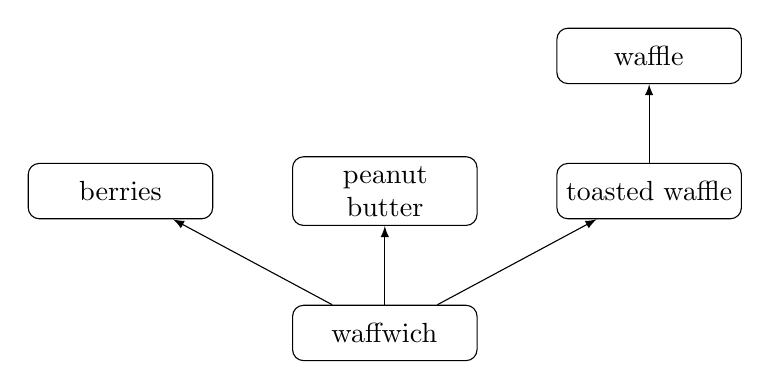
\begin{tikzpicture}[block/.style={rectangle, draw, text width=6em, text centered, rounded corners, minimum height=4em, minimum height=2em},
							line/.style={draw, -latex},
							node distance=1cm,
							auto]
			\node [block] (waffwich) {waffwich} ;
			\node [block, above= of waffwich] (pb) {peanut butter} ;
			\node [block, left= of pb] (b) {berries} ;
			\node [block, right= of pb] (tw) {toasted waffle } ;
			\node [block, above= of tw] (w) {waffle} ;
			\path [line] (waffwich) -- (pb) ;
			\path [line] (waffwich) -- (b) ;
			\path [line] (waffwich) -- (tw) ;
			\path [line] (tw) -- (w) ;
		\end{tikzpicture}
	\end{center}
\caption{How to make a waffwich}
\label{tikz:waffle}
\end{figure}

A graph like this is a very good way of describing a partially ordered
sequence of steps.  However, writing a graph is a really nasty way of
writing a program, so we need a better syntax for making
dependencies. The \maken{} recipe for a waffwich would look something
like \autoref{make:waffwich}.

\begin{make}{Using \maken{} to make a waffwich}{make:waffwich}
	\maker{waffwich}{toastedwaffles berries PB} \\
	\tab	spread peanut_buttter \dd on waffle \\
	\tab arrange berries \dd on waffle \dd in squares \dd half \\
	\tab cut waffle \\ 
	\tab fold waffle \\
	
	\maker{toastedwaffle}{waffle} \\
	\tab toast waffle
\end{make}

We must note: makefiles are not linear, unlike shell scripts. \texttt{toastedwaffle} does need to be created before \texttt{waffwich}, but does not need to appear before it in the script. \maken{} will fall through in the order it needs.

However, we've reached the point where we have to leave this
conceptual example because \maken{} is aware of whether something
exists or not, and whether it has to make it. It does this by assuming
that the target and dependencies are files, and by checking the dates
on those files. There are many exceptions to this; but let's accept
this simplification for the moment, and move on to a real example with files.

\section{Practical Example: Skull-stripping}

\subsection{Manipulating a single subject}

Follow along with this example. Copy directory 
\newline\texttt{/project_space/makepipelines/oasis-multisubject-sample/} \newline
to your home directory. \mymarginnote{!}{Don't forget use \texttt{cp -r} to copy all files in a directory.}

Your task is to skull strip all of these brains for subsequent use by \texttt{FSL}. However, note that first you need to reorient each image (try looking at it in \texttt{fslview}). So there are two commands you need to execute:
\bashcmd{fslreorient <subject>_raw.nii.gz <subject>_T1.nii.gz}

and
\bashcmd{bet <subject>_T1.nii.gz <subject>_T1.skstrip.nii.gz}

By default, \maken{} reads files called ``Makefile.'' According to the manual, GNU looks for \texttt{GNUmakefile}, \texttt{makefile}, and \texttt{Makefile} -- in that order -- but if you use just one convention, you are unlikely to get confused. 

Open the makefile that came with the directory you should have the following:

\begin{make}{Makefile as copied}{p1:1}
	\maker{OAS2_0001_T1_skstrip.nii.gz}{OAS2_001_T1.nii.gz} \\
	\tab bet OAS2_001_T1.nii.gz OAS2_001_T1_skstrip.nii.gz \\
	
	\maker{OAS2_0001_T1.nii.gz}{OAS2_0001_raw.nii.gz}\\
	\tab fslreorient2std OAS2_0001_raw.nii.gz OAS2_0001_T1.nii.gz
\end{make}

Play around with this. What happens when you execute \texttt{make} from the command line? What is it really doing?

Change the order of the rules. What happens? Note that by default, \maken{} starts by looking at the first target (the first thing with a colon after it). That is why, when you change the order of the rules, you get different outcomes, but \emph{not} because it is reading them one by one. It's creating a directed acyclic graph, but it has to start somewhere.

You can also tell it where to start. Delete any files that you may have created. Leave the makefile with the rules reordered. Now type:
\bashcmd{make OAS2_001_skstrip.nii.gz}

Now \maken{} starts with this target and goes on from there, working backward to figure out what it needs to do.

\subsection{Pattern rules and multiple subjects}

This is great, but so far we have only processed one subject. You can
create rules for each subject by cutting and pasting the two rules you
have and editing them. But that sounds like a huge chore. And what if
you get more subjects? Yuck.

You can specify in rules that you want to match patterns. Every file
begins with the subject identifier so you can use the \texttt{\%}
symbol to replace the subject in both the target and the
dependencies.\mymarginnote{!}{Patterns can be matched anywhere in the
  filename, not just at the beginning.} However, what do you do in the
recipe when you don't know the actual names of the file you're
presently working with? The \texttt{\%} won't work there. However, the
symbol \texttt{\$*} does. But that can get visually ugly. One common
shortcut is to use the automatic variable \texttt{\$@} to replace the
target, and \texttt{\$<} for the first dependency.


Using these new variables, our code can now be written:

\begin{make}{Pattern-matched Makefile}{p1:2}
	\maker{\%_T1_skstrip.nii.gz}{\%_T1.nii.gz} \\
	\tab bet \$< \$@ \\
	
	\maker{\%_T1.nii.gz}{\%_raw.nii.gz}\\
	\tab fslreorient2std \$< \$@
\end{make}

But try executing \texttt{make} now, with just those rules. You should
get an error that there are no targets. Note that \texttt{\%} does not
work as a wildcard as in the \bashn{} shell. If you are used to that
behavior, you might expect \maken{} will sense that you have a lot of
files with subject identifiers, and it should automatically expand the
\texttt{\%} to match them all. It will not do that, so you have to be
explicit about what you want to create.

For example, try typing:
\bashcmd{make OAS2_0001_T1_skstrip.nii.gz}

Now make has a concrete target in hand, and it can go forth and figure out if there are any rules that match this target (and there are!) and execute them. 

\maken{} will first look for targets that match exactly, and then fall
through to pattern matching.\footnote{It will use more specific rules
  before more generic ones: see the GNU \maken{} manual for more
  information on this behavior.}

It can be helpful to visualize pattern matching as a sieve that
catches and ``knocks off'' the part that it matched, leaving only the
stem. It will additionally strip any directory information when
present. For example, \texttt{\maker{foo/\%_T1.nii.gz}{\%.nii.gz}}
will work just as you would like.

\begin{figure}[h]
	\begin{center}
		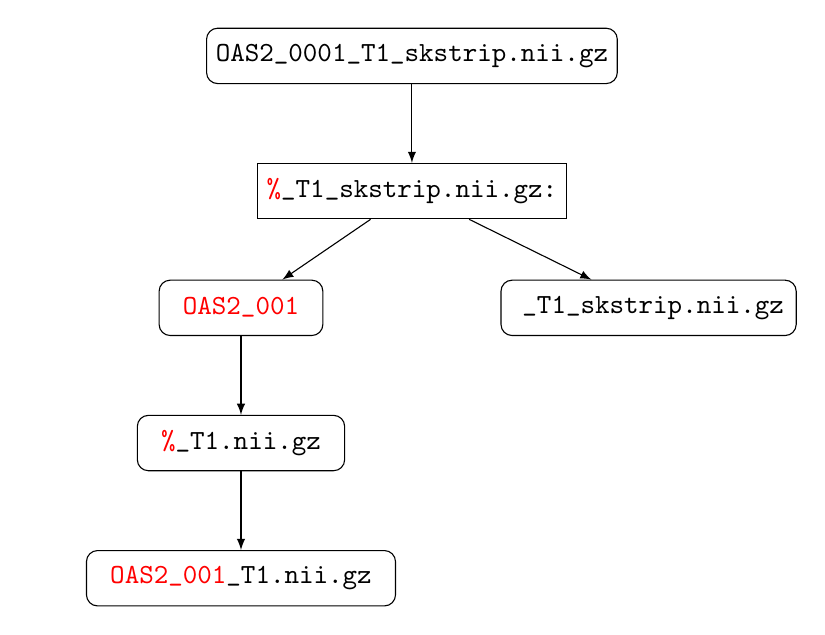
\begin{tikzpicture}[block/.style={rectangle, draw, text centered, rounded corners, minimum height=4em, minimum height=2em},
							filter/.style={rectangle, draw, text centered, minimum height=4em, minimum height=2em},
							line/.style={draw, -latex},
							node distance=1cm,
							auto]
			\node [block] (input) {\texttt{OAS2_0001_T1_skstrip.nii.gz}} ;
			\node [filter, below= of input] (filter) {\texttt{{\color{red}\%}_T1_skstrip.nii.gz: }} ;
			\node [below= of filter] (c) {} ;
			\node [text width=10em, left= of c] (t) {} ;
			\node [block, left= of c] (pattern) {\texttt{ {\color{red} OAS2_001} } } ;
			\node [block, text width=10em, right= of c] (trash) {\texttt{ _T1_skstrip.nii.gz } } ;
			\node [block, below= of pattern] (newm) {\texttt{ {\color{red} \%}_T1.nii.gz } } ;
			\node [block, below= of newm] (news) {\texttt{ {\color{red} OAS2_001}_T1.nii.gz } } ;
			\path [line] (input) -- (filter) ;
			\path [line] (filter) -- (pattern) ;
			\path [line] (filter) -- (trash) ;
			\path [line] (pattern) -- (newm) ;
			\path [line] (newm) -- (news) ;
		\end{tikzpicture}	
	\end{center}
	\caption{Pattern-matching as a sieve}
	\label{p1:sieve}
\end{figure}

\autoref{p1:sieve} shows how \maken{} identifies a pattern from an input and applies it to match the dependencies. Here, you can see that it is important to not include trailing (or leading!) underscores or other characters in your expected pattern.

\subsection{Phony targets}

Great, but how do you specify that you want to build all of these
subjects? You can create a phony target (best placed at the top) that
specifies all of the targets you really want to make. It is called a
phony target because it does not refer to an actual file.
\makecmd{\maker{skstrip}{OAS2_001_T1_skstrip.nii.gz OAS2_0002_T1_skstrip.nii.gz}}

Add as many subjects as you're patient enough to type and execute
\bashcmd{make skstrip}

Of course, typing out all the subjects (especially with ugly names
like \texttt{OAS2_001_T1_skstrip.nii.gz}) is almost as time-consuming
as copying the rule multiple times. Thankfully, there are a lot of
ways to create lists of variables, shell commands, wildcards, and most
other things you might think of. Conveniently, there is a file called
\texttt{subjects} in this directory. We can get a list of subjects by
using the following \maken{} command.  
\makecmd{SUBJECTS=\$(shell cat  subjects)}

Now we can write a target for skullstripping.
\makecmd{\maker{skstrip}{\$(SUBJECTS:=_T1_skstrip.nii.gz)}}

You also now must notify \maken{} to tell it that \texttt{skstrip} is not a real  file. Do this by using the following statement:
\makecmd{\maker{.PHONY}{skstrip}}

The pattern substitution for changing subjects to files comes from section 8.2 of the GNU \maken{} manual. You can look up the other options, but the basic function of this command is to add the affix \texttt{_T1_skstrip.nii.gz} to each item in \texttt{SUBJECTS}. 

The command uses the more general syntax, which can be used to remove parts of names before adding your new affix.
\makecmd{\$(var:suffix=replacement)}

As an esoteric example, this command could be used to replace all the final 5s with the string ``five.''
\makecmd{\$(SUBJECTS:5=five)}

\maken{} should now fail and tell you that there is no rule to make the target \texttt{OAS2_00five_T1.nii.gz}.

\subsection{Secondary targets}

Now if you type \maken{} here it is going to go through and do everything, if there's anything to do. But it's easier to see the point of secondary targets if you use the \texttt{-n} flag for \maken{}, which asks \maken{} to tell you what it's going to do, without actually doing it.\footnote{Trevor likes to use \texttt{make <cmd> -n}, which makes it easier to hit <UP> and remove the flag without any annoying arrowing around.} It's puzzling, isn't it, that all the T1 files are deleted? What's wrong here?

Because we explicitly asked for the skull-stripped brains, which \maken{} figured out it needed to make the T1 brains. This is an \emph{implicit} call. \maken, once it has finished running, goes back and erases anything that was implicitly created. This is a good thing, or a weird thing, depending on how you look at it. You can specify to \maken{} to keep those intermediary targets by adding it to the \texttt{.SECONDARY} target, like so:
\makecmd{\maker{.SECONDARY}{\$(SUBJECTS:=T1.nii.gz)}}

An alternative method is to pass any targets you want to keep to the phony variable.
\makecmd{\maker{skstrip}{\$(SUBJECTS:=_T1_skstrip.nii.gz) \$(SUBJECTS:=_T1_skstrip.nii.gz)}}

This is a little easier to interpret, as well. It also provides the advantage of allowing \maken{} to realize when an intermediary target needs to be remade. For example, if you erased only a T1 image (perhaps to rerun \texttt{bet}), and told it to \texttt{make skstrip}, it would look and see that all the T1_brain images are newer than the raw images, and therefore, no change needs to be made. While this problem could be solved by also removing the T1_brain image, that's more work and we want to do as little of that as possible.

\subsection{\texttt{make clean}}

What if you want to clean up your work? You've been deleting files by hand, but with phony targets, you don't have to. A common thing is to create a target called \texttt{clean}, which removes everything that the makefile created to bring the directory to its virgin state.

\begin{make}{\texttt{make clean}}{p1:clean}
	\maker{clean}{}\\
	\tab rm -f *T1_skstrip.nii.gz *T1.nii.gz
\end{make}

Note that in the recipe, it's totally fine to use wildcards, the recipe is executed in a shell. Also note the use of the \texttt{-f} flag. In this instance, it hides error messages from attempting to erase nonexistent files. Be very careful in its use, however.

This convention also only enforces discipline; you need to add every new file that you create in a makefile to the clean target. More dangerous is the that sometimes to get a neuroimaging subject to a certain state, you need to do some handwork that would be expensive to recreate. For example, no one wants to blow away freesurfer directories after doing hand editing. 

For these reasons, there exists the looser convention of \texttt{mostlyclean}, which means to remove things that can easily be regenerated, but to leave important partial products (e.g., your images converted from dicoms, freesurfer directories, final masks, and other things).

Also add \texttt{clean} to your list of phony targets:
\makecmd{\maker{.PHONY}{skstrip clean}}
	% Overview of make
	\chapter{\maken{} in Context}
\label{sec:practicum2}

Learning objectives: Organize a subject directory, run make in parallel, convert a shell script to a makefile.
\section{Lecture: Organizing Subject Directories}

In practice, a project will involve multiple subjects, each with
several types of scans. One could imagine a universal standard where
every nifti file contained information about where it came from and
what information it contained, and all neuroimaging programs
understood how to read and interpret this information. We could dump
all of our files into a database and extract exactly what we
wanted. We wouldn't need to use something as archaic as \maken{} because
we could specify dependencies based on the products of certain
processing steps, no matter what they were called.

If you can't imagine this, that's totally fine, because it's a very
long way off and won't look like that when it's here. Right now, we
need to work with UNIX file naming conventions to do our processing.

Therefore, selecting good naming conventions for files and for
directories is key. \maken{} specifically depends upon naming
conventions so that people can keep track of what programs and steps
were used to generate what projects. See \nameref{chap:context} for examples of good file naming conventions and typical project directory structures. 

% It's ok here to reprint modified info from Chapter 2 

Many of our studies are longitudinal. Even if they don't start out
that way, if you are trying to study a developmental or degenerative
disease, and you scan subjects once, it is often beneficial to scan
them again to answer new questions about longitudinal
progression. However, this aspect of study design poses some
challenges for naming conventions. 

Different sites organize data in different ways. For example, the
Waisman Brain Imaging Lab has a \href{http://brainimaging.waisman.wisc.edu/~oakes/teaching/directory_structure.html}{detailed description of their
preferred data organization}. 
Because our directory structure evolved from a large longitudinal
study with cross-sectional and longitudinal analyses, we
organize multiple visits for each subject as subdirectories under that
subject's main data directory. However, this organization is highly
inconvenient for processing with \maken{}.  

These basic issues and the goal of minimizing complexity drive the
directory structure described in this practical.


\section{Practical Example: A More Realistic Longitudinal Directory Structure}

\subsection{Organizing Longitudinal Data}

Follow along with this example. Copy directory 
\newline\texttt{\$MAKEPIPELINES/oasis-longitudinal-sample-small/} \\
to your home directory using the following command:
\bashcmd{cp -r \$MAKEPIPELINES/oasis-longitudinal-sample-small/ ~}

This is a very small subset of the OASIS data set (\texttt{http://www.oasis-brains.org}), which consists of a
longitudinal sample of structural images. There are several T1 images
taken at each scan session, and several visits that occurred a year or
more apart. I have reduced the size of this directory by taking only one of the T1 images
for each person, for each visit, and only of a small sample of
subjects.

Look at the directory structure of \texttt{subjects/}. A useful command to do this is called \texttt{find}. For example, if you are in the \texttt{subjects} directory you can type:
\bashcmd{find .}

You can see that as we have discussed, each subject has one to five
separate sessions. The data for each session (here, only a single
MPRAGE) is stored under each session directory. I realize that
creating a directory to store what is right now a single scan seems a
bit like overkill, but in a real study there would be several types of
scans in each session directory. Here, to focus on the directory
organization and how to call make recursively, we are only looking at
one type of scan.

Normally there are two types of processing that are performed for a
study. The first are subject-level analyses --- in short, analyses that
are completely independent of all the other subjects. The second are
group-level analyses, or analyses that involve all the subjects
data, or a subset of the subjects. In general, a good rule of thumb is that the results of
subject-level analyses are best placed within the subject directories.

Group-level analyses seem to be best found elsewhere in the project
directory, either as a subdirectory within a specific timepoint or organized at the top
level.

Create the directory \texttt{visit1/} within your copy of \texttt{oasis-longitudinal-sample-small}. 
\bashcmd{mkdir visit1}

Now \texttt{cd} into it:
\bashcmd{cd visit1}

What we want to do is create the symbolic links for each subject's first visit here. 

You can do one link by hand:
\bashcmd{ln -s ../subjects/OAS2_0001/visit1 OAS2_0001}

This command symbolically links the directory \texttt{../subjects/visit1/OAS2_0001} to the original directory \texttt{../subjects/OAS2_0001/visit1}. 
\mymarginnote{!}{Your \texttt{ls} command may be aliased to something pleasing, in which case you might see slightly different behavior than described here.} 
Now, if you enter \texttt{ls -l} into the command line while remaining in the \texttt{visit1} directory, you will notice that the subdirectory \texttt{OAS2_0001} is symbolically linked, as indicated by an arrow, to the original target directory. You can also check whether a file or directory is linked by using the \texttt{ls -F} shorthand command, which indicates symbolic links with an\@ symbol. The command \texttt{ls -L} dereferences the symbolic links so that you can view information for the original target file or directory itself.

You can also create symbolic links in bulk. To do so, remove the link that you have just created and
use the program in the \texttt{visit1} directory (\texttt{makelinks}) to create all the subject links for visit1. 
\mymarginnote{!}{The current directory won't be in your PATH, so make sure to call it with \texttt{./makelinks}.}

Take a look at the \texttt{makelinks} script, reprinted below. This script loops through all of the subject directories that have a first visit (visit1). It extracts the subject identifier from the directory name (\texttt{\$i}) by using the \texttt{egrep} command to find the bit of the name that matches the subject identifier pattern (\texttt{OAS2_[0-9]}). With this information, it can link the subject name to the directory. 

\begin{bash}{Script to create symbolic links within a longitudinal
    directory structure}{bash:links}
\#!/bin/bash

for i in ../subjects/*/visit1\\
do\\
\tab	subject=`echo \$i| egrep -o 'OAS2_[0-9]*'` \\
\tab	ln -s \$i \$subject\\
done\\
\end{bash}

\subsection{Recursive \maken{}}
Now let's look at the Makefile (\texttt{visit1/Makefile}).  This is just a 
top-level ``driver'' makefile for each of the subjects. All it does is
create a symbolic link, if necessary, to the subject-level makefile,
and then it goes in and calls \maken{} in every subdirectory.

Do you know why is the subject target a phony target? The reason is
that we want \maken{} to be triggered within the subject directory every
time we call it.

Create the symbolic links to the subject-level makefile as follows:
\bashcmd{make Makefile}

Do you know why we use the \texttt{\$PWD} variable to create the link?
If we used a relative path to the target file, what would happen when
we go to the subject directory?

Let us see how this works. Look at the subject-level makefile (\texttt{Makefile.subdir}). Go into
a subject directory and run \texttt{make}.

By now, you might be getting really tired of seeing the same \texttt{fslreorient2std} and \texttt{bet} commands. \maken{}, by default,
will echo the commands that it executes to the terminal. If you would
like it to stop doing that, you can tell it not to do that by
prepending the \texttt{@} character to each line.
\begin{lstlisting}
	%_T1_skstrip.nii.gz: %_T1.nii.gz
		@bet $< $@
\end{lstlisting}
%\begin{make}{The \texttt{@} character hides commands}{}
%\maker{\%\_T1\_skstrip.nii.gz}{\%\_T1.nii.gz}\\
%  \tab @bet \$< \$@
%\end{make}

Now go find the same subject via the subject subtree:
\bashcmd{cd ~/oasis-longitudinal-sample-small/subjects/visit1/OAS2_0001/visit1}

Type \texttt{make} and see that it works. Part of this magic is that we set
the subject variable correctly, even though where it appears in a
directory path is different in each place.

There is a useful little rule defined in the GNUMake Cookbook (Chapter
2, p. 44) that may be useful for checking that you have set variables correctly. Add the following lines to the subject-level makefile.

\begin{lstlisting}
	print- %:
		@echo $* = $($*)
\end{lstlisting}
%\begin{make}{Printing out the value of variables}{}
%\maker{print-\%}{}\\
%\tab @echo \$* = \$(\$*)
%\end{make}

Now if you type: \bashcmd{make print-subject} \\
You can see the value that the variable \texttt{subject} is set to. Note that even if you place this new rule at the very top of the makefile, it will not execute this rule by default. It will fall through to the next non-pattern rule. This is one of the ways in which pattern rules (implicit rules) differ subtly from explicit rules. 

\subsection{Running \maken{} over multiple subject directories}
Now that we have verified that the individual makefile works, we can
go to the \texttt{visit1} directory and process all the
subjects. First, go back and edit the subject-level makefile to remove
the \texttt{@} characters in front of the commands so that they are
printed.

From within the \texttt{visit1/} directory, type:
\bashcmd{make -n TARGET=skstrip}

Note that what this is doing is (recursively) going into each subject directory and calling \maken{}. It will do this whether or not there is anything to do within the subject directory, because each subject directory has no dependencies. However, because we have specified the \texttt{-n} flag, it prints out what commands it will perform without actually executing them.

We can do this work in parallel. Bring up a system monitor (\texttt{gkrellm} is installed on the IBIC systems). See how many processing units you have and how busy they are. Note these numbers and get familiar with the configuration of the computers that you have in the lab. In general, each job will require a certain amount of memory and can use at maximum one CPU. A safe calculation for most things is that you can normally run as many jobs at one time on a computer as you have CPUs. This is a huge oversimplification but it will suffice for now. 

You can specify to make how many CPUs to use. For example, if we specify the \texttt{ -j} flag with an argument of 2 (processors), we can parallelize execution of \maken{} over two CPUs. 
\bashcmd{make -j 2 TARGET=skstrip}

If you specify \texttt{make -j} without any options, it will use as many CPUS as  you have on your machine. This is great if all the work you have ``fits'' into the computing resources that are available. However, if it does not, you can use a computing cluster.

In our environment, we use the Sun Grid Engine (SGE) to distribute
jobs across machines that are ``clustered'' together. To run on a
cluster, you need to be logged on one of the machines that is allowed
to submit to the grid engine.\footnote{In IBIC, they are:  \texttt{broca}, \texttt{dentate}, \texttt{homunculus}, \texttt{pole}, \texttt{pons}, \texttt{precuneus}, and \texttt{triangularis}.} Once there, you can use the command:
\bashcmd{qmake -cwd -V -- -j 20 TARGET=skstrip}

Here, we use \texttt{qmake} instead of \texttt{make} to interact with the grid engine. The \texttt{-cwd} flag says to run from the current working directory, and \texttt{-V} says to pass along all your environment variables. You will normally want to specify both of these flags. The \texttt{--} specifies to \texttt{qmake} that we are done specifying \texttt{qmake} flags and are now giving normal flags to \maken{}. For example, in this command we specify 20 jobs. 

As an optional exercise, here you might want to set up the same directory structure for \texttt{visit2/} and build everything from scratch in parallel.

\subsection{Running FreeSurfer}
Now let us look at an example of a subject-level analysis that we typically don't run within the subject directories. FreeSurfer \citep[see][]{Desikan2006968, Fischl01012004, Fischl2004S69} is a program that we use for cortical and subcortical parcellation. It itself is a complicated neuroimaging pipeline that is built using \maken{}. It likes to put all subject directories for an analysis in one directory, which makes it difficult to enforce the subject-level structure described. But in general, it is much wiser to work around what the programs want to do than to reorganize their output in ways that might break when the software is updated! This is our approach.

The FreeSurfer example is documented in \nameref{example:freesurfer}. 

% For complete FreeSurfer references, add these: Fischl26092000, FischlLiuDale, FischlSalat2002, HBM:HBM10, Jovicich2006436, Kuperberg2003, Rosas12032002, Salat2004, Segonne20041060, dale:99, fischl:99, han:06, sledzijdenbos1998, spf2007, reuter:robreg10, reuter:bias11, reuter:long12
 	% Make in context
	
	\chapter{Documenting a makefile for this manual}

This chapter will show you how to document (in \LaTeX) a makefile for this manual. While \LaTeX{} may look intimidating if you haven't used it before, it is fairly straightforward to use. We have created a number of tools to help you insert your makefile into this manual.

\section{Makefile to \LaTeX}

There are a number of things that need to be changed in a bare makefile in order to import it to the \LaTeX{} structure used for this manual. To do the basic stuff, call the script \texttt{makeToTex}\footnote{Please report bugs to Trevor at \url{tkmday@uw.edu}.} on your makefile(s). It can accept any number makefiles and outputs \texttt{<file>_texed.txt}. It has two flags, \texttt{h} and \texttt{v}, which call the help menu and verbose mode, respectively.

There are two main things that need to happen: certain symbols need to be escaped in \LaTeX, and recipes need to be formatted in a  macro to make them pretty. Symbols like ``\$'' and ``\mypound'' have special functions in \LaTeX, and will result in catastrophe if you don't fix them.

The functionality of the script is documented in \autoref{appendix:makeToTex}. Please refer to it if you have any troubles.

Now to bring your new makefile into a \LaTeX document!

\section{Editing a .tex File}

Any script compiled with the main document will include the necessary environment \texttt{makefileread}. In your \LaTeX document, create a newline, ensuring the indentation is consistent and insert the command \verb!\begin{makefileread}!. If you are using a \LaTeX editor, it may autocomplete with the last line, \verb!\end{makefileread}.! If not, you'll have to type it yourself.

Paste your code between those two commands. It should be one level more indented.

To insert text comments between sections of code, you may terminate the environment, add your text and begin a new environment with the rest of the code. Refer to the style guide (\autoref{appendix:sg}) for stylistic choices we use to keep our text consistent. There are many idiosyncrasies to \LaTeX, too many to go into here, but a few of note:

\begin{easylist}[itemize]
	& Quotes are written with two backticks (opening) or two apostrophes (closing).
	& Please leave a blank line between paragraphs. 
	& Special characters should always be escaped (see \autoref{appendix:makeToTex} or Internet resources).
\end{easylist}

Feel free to scroll through chapter files to look for examples of usage if you are in doubt. The answers to further questions can probably be found online (I especially like \url{http://tex.stackexchange.com}).

\section{How Makefile Documentation Should Look}

Notice how documentation will begin on a new page and a new page will be created at the end of the documentations. This is necessary to allow for wider margins that make the code easier to read.

\newgeometry{scale=0.85, centering}

\begin{minted}[gobble=1]{make}
	# act-plus freesurfer makefile
	
	# This is where the subject directories live 
	PROJHOME=/projects2/act-plus/subjects/session1
	
	cwd=$(shell pwd)
	
	SUBJECTS=$(shell cat /projects2/act-plus/uds/good_subjects.txt)
	#SUBJECT=$(notdir $(cwd))
	
	# Set open MP number of threads to be 1, so that we can parallize using make.
	export OMP_NUM_THREADS=1
	
	# for Freesurfer (running version 5.3)
	export SUBJECTS_DIR=/projects2/act-plus/freesurfer
	export QA_TOOLS=/usr/local/freesurfer/QAtools_v1.1
	
	# be really careful with paths and variables - two versions of freesurfer
	# installed
	export FREESURFER_SETUP = /usr/local/freesurfer/stable5_3/SetUpFreeSurfer.sh
	export RECON_ALL = /usr/local/freesurfer/stable5_3/bin/recon-all $(RECON_FLAGS)
	export TKMEDIT = /usr/local/freesurfer/stable5_3/bin/tkmedit
	
	define usage
	@echo Usage:
	@echo "make, or make interactive	Makes interactive targets"
	@echo "make noninteractive		Makes noninteractive targets"
	@echo 
	@echo Noninteractive targets:
	@echo "make setup		Copies source files to this directory"
	@echo "make freesurfer	Runs freesurfer"
	@echo
	@echo Other useful targets:
	@echo "make clean		Remove everything! Be careful!"
	@echo "make mostlyclean		Remove everything but the good bits."
	@echo "make help		Print this message."
	@echo
	@echo Variables:
	@echo "RECON_FLAGS	Set to flags to recon-all, by default"
	@echo "WAVE		1, 2 or 3 to select subjects, for setup"
	endef
	
	export SHELL=/bin/bash
	
	.PHONY: qa clean mostlyclean output noninteractive 
	
	noninteractive: setup freesurfer
	
	all: noninteractive
	
	output=$(SUBJECTS:%=%/mri/aparc+aseg.mgz) $(SUBJECTS:%=%/mri/brainmask.nii.gz)
	freesurfer: $(output)
	
	#recon-all $(RECON_FLAGS) -subjid  $${subj} -FLAIR $${subj}/flair.nii.gz -FLAIRpial;\
	
	#####################################
	
	qafiles=$(SUBJECTS:%=QA/%)
	
	qa: $(qafiles)
	
	QA/%: %
	source $$FREESURFER_SETUP ;\
	$(QA_TOOLS)/recon_checker -s $*
	
	#####################################
	
	%/mri/aparc+aseg.mgz: $(PROJHOME)/%/memprage/T1.nii.gz
	rm -rf `dirname $@`/IsRunning.*
	source /usr/local/freesurfer/stable5_3/SetUpFreeSurfer.sh ;\
	export SUBJECTS_DIR=$(SUBJECTS_DIR) ;\
	/usr/local/freesurfer/stable5_3/bin/recon-all -i $< -subjid $* -all ;\
	/usr/local/freesurfer/stable5_3/bin/recon-all -s $* -T2 
		$(PROJHOME)/$*/flair/Flair.nii.gz -T2pial
		
	%/mri/brainmask.nii.gz: $(SUBJECTS_DIR)/%/mri/aparc+aseg.mgz
	source /usr/local/freesurfer/stable5_3/SetUpFreeSurfer.sh ;\
	mri_convert $(SUBJECTS_DIR)/$*/mri/brainmask.mgz $@
	
	clean:
	echo rm -rf $(inputdirs)
	
	mostlyclean:
	@echo "Here I would delete things that are not necessary after all is said and done."
	
	output: 
	@echo "Nothing yet"
	
	setup: $(SUBJECTS)
	
	%:  $(PROJHOME)/%/memprage/T1.nii.gz 
	mkdir -p $@/mri/orig; \
	cp $^ $@/mri/orig; \
	cd $@/mri/orig; \
	mri_convert T1.nii.gz 001.mgz
	
	help:
	$(usage)
	
	
\end{minted} % How to document makefiles
	
	\appendix
	
	\chapter{\texttt{makeToTeX}}
\label{appendix:makeToTex}	
	
In case your script gives \LaTeX problems, the steps \texttt{makeToTex} undertakes are listed here.
	
\vspace{0.5\baselineskip}\hrule\vspace{0.5\baselineskip}
	
\begin{easylist}[enumerate]
	& \texttt{;\textbackslash} is replaced with \texttt{;}\verb!\textbackslash!
	& Covert any recipes to a special command to turn the target blue.
	& Strip comments (lines beginning with \texttt{\#}).
	&& At present, it doesn't strip trailing comments. Please remove those yourself.
	& Escape the characters \texttt{\$}, \texttt{\%}, and \texttt{\#}.
	& Add the terminal newline command (\texttt{\textbackslash\textbackslash}) to non-blank lines.
	& Replace \textasciicircum with \verb!\textasciicircum!.
	& Replace double dashes (\dd) with a macro that stops it from turning them into hyphens (--).
	& Replace single TAB characters with a macro.
	& Replace multiple TAB characters with \verb!\hfill!, a \LaTeX command that spaces nicely.
	& Leading and trailing quotes are specified differently in \LaTeX. Leading quotes are coded with a backtick and trailing with an apostrophe.
	& Extra spaces and multiple blank lines are filtered out.
	\end{easylist}
	
	
\vspace{0.5\baselineskip}\hrule\vspace{0.5\baselineskip}
	
Please ensure all comments are removed! They are very troublesome to display.
	
\chapter{Style Guide}
\label{appendix:sg}
	
Please refer to this guide when in doubt. It covers typographic and phrasing consistencies.
	
\begin{easylist}[enumerate]
	& Monospace (use the \verb!\texttt{}! macro) the following things:
	&& \maken, when referring to the program.
	&&& Use the macro \verb!\maken{}!. To remove the trailing space (for example, to use a comma after \maken), call the macro without the braces, \verb!\maken!.
	&&& Never uppercase.
	&& \bashn
	&&& Use the macro \verb!\bashn{}!.
	&& Any \bashn{} or \maken{} command. This is done automatically in the one-liner and multi-line environments. Be sure to monospace commands written in-line.
	&& Explicit references to a file: e.g., ``\ldots open \texttt{subjects.txt}.''
	&& Commands run from the command line: e.g., \texttt{ls}, \texttt{bet}, \texttt{flirt}, \texttt{qmake}, etc \ldots
	&& References to directories: e.g., \texttt{/bin/}, \texttt{oasis-multisubject-sample/}.
	&&& Use the trailing slash for clarity in all cases.
	&& References to named variables: e.g., \texttt{\$(SUBJECTS)}, \texttt{\$<}, \texttt{\%}, \texttt{\$PWD}.
	&& Command-line flags written in-line: e.g., \texttt{-n}, \texttt{-lart}.
	& Don't monospace:
	&& \textbf{Don't double up on quotes and monospacing.} If both would be used, prefer quotes. This is to avoid a complete monospacing overload.
	&& Abstractions or filetypes: e.g., ``Makefiles are usually located \ldots'' or ``The nifti files \ldots''
	&& Programs typically used through a GUI: e.g. OpenOffice, gimp.
	&& Tool suites, like FSL or AFNI.
	&& The names of operating systems.
	&& References to the grid engine in any form.
	&&& Use the article with the abbreviation: ``the SGE.''
	&&& ``Grid engine,'' not ``gridengine.'' This is Oracle/SG's usage, although they capitalize it, which we won't do.
	&& Subject identifiers.
	& Oxford comma = yes: e.g. ``X, Y\textcolor{red}{,} and Z,'' not ``X, Y and Z.''
	& Don't use em dashes (--) for emphasis. They should appear in pairs the majority of the time.
	& Margin notes and footnotes:
	&& Use margin notes to call out things a new reader would find useful:
	&&& Define important terms with a [?].
	&&& Call out important notes with a [!].
	&& Use footnotes for things that could be completely ignored: advanced features, humorous commentary, etc\ldots.
	& \LaTeX{} swallows up two dashes (\dd). Use \verb!\dd! to get a double dash. You can use a space after this command and \LaTeX will ignore it.
	& \textbf{Skull-strip:} Two words, always hyphenated.
	& Headers:
	&& Chapters and Sections Are in Title Case
	&& Subsections in sentence case
	&& Figure captions in sentence case
	& Numerals:
	&& Spell out numbers less than 10, except the ones \LaTeX{} generates.
	&& Always spell out a number at the beginning of a sentence. However, it usually better to recast the sentence to avoid this.
	&& If you must refer to multiple number things, try:
	&&& Using A, B, C \ldots{} instead: ``Process A will overwrite foo.out just in time for process B to use it.''
	& Plurals
	&& Since we may have to pluralize some weird things: No apostrophe between the stem and the ``s,'' no matter what. Use the same formatting (e.g. monospacing). If possible, recast the sentence.
	& M/makefile
	&& ``a makefile'' is an abstract noun referring to any make script (cf. ``a shell script''). This should be capitalized when appropriate.
	&& ``the Makefile'' is the top-level makefile in a directory, usually named \texttt{Makefile} by IBIC conventions. This reference to the file with the same name does not need to be monospaced.
	& Backticks and single quotes in monospaced font:
	&& Use \texttt{\textbackslash\`{}\{\}} to get the correct backtick symbol.
	&& There is currently no support for a straight single quote in the defaulty \verb!\ttfamily! font or Inconsolata at present.
	& Ellipses
	&& Spaces before and after: ``this \ldots{} and that.''
	&& Use \verb!\ldots!
	& FreeSurfer
\end{easylist}

		
\end{document}